%%%%%%%%%%%%%%%%%%%%%%%%%%%%%%%%%%%%%%%%%%%%%%%%%%%%%%%%%%%%%%%%%%%%%%%%%%%%%%%%
%2345678901234567890123456789012345678901234567890123456789012345678901234567890
%        1         2         3         4         5         6         7         8

%\documentclass[letterpaper, 10 pt, conference]{ieeeconf}  % Comment this line out
% if you need a4paper
%\documentclass[a4paper, 10pt, conference]{ieeeconf}      % Use this line for a4
% paper



% The following packages can be found on http:\\www.ctan.org
%\usepackage{graphics} % for pdf, bitmapped graphics files
%\usepackage{epsfig} % for postscript graphics files
%%\usepackage{mathptmx} % assumes new font selection scheme installed
%%\usepackage{times} % assumes new font selection scheme installed
%%\usepackage{amsmath} % assumes amsmath package installed
%%\usepackage{amssymb}  % assumes amsmath package installed
%\usepackage{subfigure}
%\usepackage{float}
%
%\restylefloat{figure}

\title{\LARGE \bf
	The effect of limb position on myoelectric prosthetic control using linear regression
}%final name

%\author{ \parbox{3 in}{\centering Huibert Kwakernaak*
%         \thanks{*Use the $\backslash$thanks command to put information here}\\
%         Faculty of Electrical Engineering, Mathematics and Computer Science\\
%         University of Twente\\
%         7500 AE Enschede, The Netherlands\\
%         {\tt\small h.kwakernaak@autsubmit.com}}
%         \hspace*{ 0.5 in}
%         \parbox{3 in}{ \centering Pradeep Misra**
%         \thanks{**The footnote marks may be inserted manually}\\
%        Department of Electrical Engineering \\
%         Wright State University\\
%         Dayton, OH 45435, USA\\
%         {\tt\small pmisra@cs.wright.edu}}
%}

\author{Simon Bruun, Oliver Thomsen Damsgaard, Martin Alexander Garenfeld, Irene Uriarte}% <-this % stops a space

%\begin{document}

\setcounter{topnumber}{6}
\setcounter{bottomnumber}{6}
\setcounter{totalnumber}{10}
\renewcommand{\topfraction}{1}
\renewcommand{\bottomfraction}{1}
\renewcommand{\textfraction}{0}
\renewcommand{\floatpagefraction}{1}
		
	\maketitle
	\thispagestyle{empty}
	\pagestyle{empty}
	
	\begin{multicols}{2}

	%%%%%%%%%%%%%%%%%%%%%%%%%%%%%%%%%%%%%%%%%%%%%%%%%%%%%%%%%%%%%%%%%%%%%%%%%%%%%%%%
	\begin{abstract}
%		Electromyography (EMG) is widely used for controlling functional prosthetics. However, EMG signals for the same movements change with variations in limb position and lowers the accuracy in control schemes \cite{fougner2012}. Most of the previous studies have utilized classification for pattern recognition when changing limb position, with a negative effect in performance. %Linear regression is a newer method in control of myoelectric prosthetics, which has proven to yield robust simultaneous and proportional control \cite{hanhe2014}. %Only the RMS feature was previously tested in variations of limb positions in regression-based control \cite{hwang2017}. 
This study investigated the effect of limb position in a linear regression-based control scheme, when using 
%the commonly used 
Mean Absolute Value (MAV) and Logarithmic Variance (LogVar) as features. %where the latter has shown linear properties \cite{hanhe2014}.
Seven (more now) able-bodied subjects were recruited for data acquisition, performing four wrist movements in three different limb positions. One regression model was build to recognize the different wrist movements under study, taking into account both features. %One regression model %(regressor) 
%was build for each wrist movement for each test subject: four for each feature. 
The regressors were tested online in a virtual environment. %where the time to complete a target-reaching task of sixteen targets was measured. %The performance (time per reached target) of the online test was compared between the different limb positions of the same feature and between all limb positions of the two features through statistical analysis. 
%Using a Friedman's test the performance scores between the three limb positions prove not to be significantly different 
%(p = 0.5647), 
%when applying the LogVar trained regressors %in the online test. For the MAV trained regressors the performance score between all limb positions cannot be proven significantly different either (p = 0.1561). 
%There was no difference in the time to reach the targets across the two features %(LogVar: 6.5 s, MAV: 5.5 s; p = 0.13).
The results showed that changes in limb position do not affect the control when linear regression model is trained with the %MAV or LogVar 
features extracted. This is opposed to previous studies using classification as control scheme. Linear regression has the potential to be used in future control schemes for myoelectric prosthetics for use in daily life tasks.\\


\textit{\textbf{Keywords---}}surface electromyography, inertial measurement unit, simultaneous and proportional myoelectric control, regression, hand motion classification, hand prosthetic


Electromyography (EMG) is widely used for controlling functional prosthetics. However, EMG signals for the same movements change with variations in limb position and lowers the accuracy in control schemes \cite{fougner2012}. Most previous studies testing the effect of limb position, have utilized classification for pattern recognition with a negative effect in performance. This study investigated the effect of limb position in a linear regression-based control scheme, when using Mean Absolute Value and Logarithmic Variance as features, and including IMU data to improve the performance of the regression models. 12 able-bodied subjects were recruited for data acquisition, performing four wrist movements in three different limb positions. One regression model was build to recognize the different wrist movements under study, taking into account both features. The regressors were tested online in a virtual environment. The results showed that changes in limb position do not affect the control when linear regression model.
This is opposed to previous studies using classification as control scheme. Linear regression has the potential to be used in future control schemes for myoelectric prosthetics for use in daily life tasks.\\
		
\textit{\textbf{Keywords---}}surface electromyography, inertial measurement units, simultaneous and proportional myoelectric control, linear regression, lower arm prosthetics.
	\end{abstract}
	
	%%%%%%%%%%%%%%%%%%%%%%%%%%%%%%%%%%%%%%%%%%%%%%%%%%%%%%%%%%%%%%%%%%%%%%%%%%%%%%%%
	
\section{INTRODUCTION}%%%%%%%%%%%%%%%%%%%%%%%%%%%%%%%%%%%%%%%%%%%%%%%%%%%%%%%%%%%%%%
		
%		%What has been done in the EMG-prosthesis area?
In recent years the development of EMG controlled lower arm prosthetics has advanced considerably, due to an increased interest in the area along with higher demands for better prosthetics and more precise control. \cite{Fougner2012} In the early years most EMG prosthetics functioned by controlling one degree of freedom (DOF) with on-off control, mainly by linking antagonistic muscles to one DOF. This kind of prostheses change between states due to a switching impulse which cause a state machine to shift its present state. Usually a strong and fast muscle contraction from the users is employed to generate the switching signals. \cite{amsuess2014}
This type of control provided users a way to control more than one DOF, but never simultaneously. The switch-control functioned on a cycle, so users would have to go through all the movements of the prosthesis to find the one they wanted to perform. However, as demands rose, more complex methods was introduced to the EMG prosthetics scene. Classification methods effectively enabled users to use DOF's more freely because the switching was now replaced by direct recognition of different muscle contractions linked to specific prosthetic movements. This also effectively enabled proportional control of movements, but gave rise to new problems: a wider range of control would give less accurate movements, and training the classifiers proved difficult, as the training could over-fit, causing extended use of the prosthetics to degrade in performance. \cite{Ison2016}

%Regression
Introducing regression as a new mapping method in myoelectric prosthetics provided a way to enable both simultaneous and proportional control of multiple DOF's. Regression is able to provide a continuous value for each DOF based on the recorded EMG signal, while a classifier only decides upon a certain class. \cite{hahne2014, jiang2010}
This means that classification can only translate a recorded EMG signal to one movement of the prosthetic at a time. It can do so proportionally but the handling still lacks natural control, since movements by able-bodied individuals very rarely only happen in one DOF at a time. Regression methods constantly provide a value, and since several regressors can be used at a time, several values can be used in the recognition of movements. This is what enables regression methods to perform simultaneous and proportionally. 

Applying regression as a mapping method in proportional and simultaneous control of multiple DOF's has been shown to perform well in recognition of movements and doing so with a low computation time. \cite{hahne2014} However, very few studies have tested the regressor performance in daily life tasks outside the clinical training environment. \cite{jiang2012} A study by Fougner et al. \cite{Fougner2011} has addressed the problem that most studies test their method on only one limb position. This means that the actual performance of regression methods has not yet been properly addressed when recognizing movements, where the arm changes position during daily life tasks. 

%Which issues are there in the EMG-prosthesis area?(decreasing quality of control of hand gestures when the arm is placed in different positions)
When recording EMG signals it has been shown that some muscles are activated based on joint angles, even though the muscles are not involved in the movement of that joint \cite{Fougner2011}. This provides a problem, but can be explained by muscle-synergies \cite{DeRugy2013}. These muscle-synergies are created by the Central Nervous System (CNS) and coordinated into activation of different muscles at varying times. This enables the CNS to control the muscle-synergies instead of controlling each muscle individually to perform movements \cite{jiang2009}. This means that muscles in the lower arm can be activated when muscles in the upper arm are activated, in a level that will be detectable in EMG recordings, and enough to alter recognition of movements, when the arm is active in limb positions other than those tested in a clinical environment. 

%What would be novel to add to this area?(adding IMU’s to a regressor, since it has been done with a classifier)
In order to overcome the problem of muscles-synergies, Fougner et al. \cite{Fougner2011} has suggested to combine recordings of EMG signals with inertial information to provide limb position data. This could be beneficial in increasing the accuracy of EMG controlled prosthetics for use in daily life tasks. 
Even though the combination of EMG and Inertial Measurement Unit (IMU) data has been proposed as a valid way to improve the performance and accuracy of EMG based prosthetics, it has only been investigated in few studies. \cite{Roy2010, Imtiaz2014, jiang2012}

To the authors knowledge the combination of EMG recordings and IMU data has only been done with classification methods. A novel approach to further investigate the usability of combining EMG and IMU is to build a regression based control scheme for myoelectric prosthetics. This would enable both proportional and simultaneous control of several DOF's, where the inclusion of IMU data should provide more information on limb position to counter the effect of limb position.






%In recent years the development of EMG controlled prosthesis have advanced due to an increased interest in the area as well as a higher demand of better control of this prosthesis.\cite{fougner2012}
%In the early years most EMG prosthetics functioned by only controlling one DOF by \textit{on-off control}, mostly by linking antagonistic muscles to one DOF. %This along with \textit{mode switching} provided users a way to control more than one DOF, but not in a simultaneous way. 
%This control provided a way to control more than one DOF, but not simultaneously. However, as demands would rise, more complex methods were introduced to the EMG scene. Classification methods enabled simultaneous control of more than one DOF, but gave rise to new problems; a wider range of control would give less accurate movements, and training the pattern recognition methods proved difficult, as the training could over-fit, causing extended use of the prosthetics to degrade in performance. \cite{Ison2016}.
% 
%It has been proved that regression techniques can be apply as a new mapping method to achieve simultaneous and proportional control of multiple DOFs\cite{hanhe2014}. Regression methods provide a continous value for each DOF based on the recorded EMG signal, while classification methods only decides upon a certain class. However there are still difficulties when prosthesis perform outside the clinical training environment\cite{jiang2012}.
% Fougner et al.\cite{Fougner2011} noticed that majority of studies only take in account one limb position. It has been shown that some muscles are activated based on joint angles \cite{reference}, even though the muscles are not involved in the movement of that joint, which can be explained by muscle-synergies existed between muscles.
%% which becomes a problem since muscles create muscle-synergies to perform movements. 
%Variations in limb positions can have an impact on the robustness of EMG pattern recognition. %To be able to offer a good perform of the prosthesis, these should be able to execute with the same accuracy diverse hand gestures in different limb positions. 
%In order to overcome this problem it has been suggested to combine EMG data as well as IMU data, to provide limb position information. Nevertheless this combination of data have only been investigated for classification methods. 
%In this study we test the performance of linear regression methods combining EMG and IMU data for a simultaneous and proportional control of two DOFs in a lower-arm prothesis while the arm is located in different limb positions.
%% in the training sesions of the regressor to obtain simultaneous and proportional control of EMG prosthesis. 
%%Hypotheses
%%Simultaneous and proportional control of two  DOF's of the wrist in different limb positions, can be achieve trough the use of linear regression as control system. Combining EMG and IMU's can minimize the limb position effect when using regression as control system.
In recent years the development of EMG controlled lower arm prosthetics has advanced considerably, due to an increased interest in the area along with higher demands for better prosthetics and more precise control. \cite{Fougner2012} In the early years most EMG prosthetics functioned by controlling one degree of freedom (DOF) with on-off control, mainly by linking antagonistic muscles to one DOF. This kind of prostheses change between states due to a switching impulse which cause a state machine to shift its present state. Usually a strong and fast muscle contraction from the users is employed to generate the switching signals. \cite{amsuess2014}
This type of control provided users a way to control more than one DOF, but never simultaneously. The switch-control functioned on a cycle, so users would have to go through all the movements of the prosthesis to find the one they wanted to perform. However, as demands rose, more complex methods was introduced to the EMG prosthetics scene. Classification methods effectively enabled users to use DOF's more freely because the switching was now replaced by direct recognition of different muscle contractions linked to specific prosthetic movements. This also effectively enabled proportional control of movements, but gave rise to new problems: a wider range of control would give less accurate movements, and training the classifiers proved difficult, as the training could over-fit, causing extended use of the prosthetics to degrade in performance. \cite{Ison2016}

Introducing regression as a new mapping method in myoelectric prosthetics provided a way to enable both simultaneous and proportional control of multiple DOF's. Regression is able to provide a continuous value for each DOF based on the recorded EMG signal, while a classifier only decides upon a certain class. \cite{hahne2014, jiang2010}
This means that classification can only translate a recorded EMG signal to one movement of the prosthetic at a time. It can do so proportionally but the handling still lacks natural control, since movements by able-bodied individuals very rarely only happen in one DOF at a time. Regression methods constantly provide a value, and since several regressors can be used at a time, several values can be used in the recognition of movements. This is what enables regression methods to perform simultaneous and proportionally. 

Applying regression as a mapping method in proportional and simultaneous control of multiple DOF's has been shown to perform well in recognition of movements and doing so with a low computation time. \cite{hahne2014} However, very few studies have tested the regressor performance in daily life tasks outside the clinical training environment. \cite{jiang2012} A study by Fougner et al. \cite{Fougner2011} has addressed the problem that most studies test their method on only one limb position. This means that the actual performance of regression methods has not yet been properly addressed when recognizing movements, where the arm changes position during daily life tasks. 

When recording EMG signals it has been shown that some muscles are activated based on joint angles, even though the muscles are not involved in the movement of that joint \cite{Fougner2011}. This provides a problem, but can be explained by muscle-synergies \cite{DeRugy2013}. These muscle-synergies are created by the Central Nervous System (CNS) and coordinated into activation of different muscles at varying times. This enables the CNS to control the muscle-synergies instead of controlling each muscle individually to perform movements \cite{jiang2009}. This means that muscles in the lower arm can be activated when muscles in the upper arm are activated, in a level that will be detectable in EMG recordings, and enough to alter recognition of movements, when the arm is active in limb positions other than those tested in a clinical environment. 

In order to overcome the problem of muscles-synergies, Fougner et al. \cite{Fougner2011} has suggested to combine recordings of EMG signals with inertial information to provide limb position data. This could be beneficial in increasing the accuracy of EMG controlled prosthetics for use in daily life tasks. 
Even though the combination of EMG and Inertial Measurement Unit (IMU) data has been proposed as a valid way to improve the performance and accuracy of EMG based prosthetics, it has only been investigated in few studies. \cite{Roy2010, Imtiaz2014, jiang2012}

To the authors knowledge the combination of EMG recordings and IMU data has only been done with classification methods. A novel approach to further investigate the usability of combining EMG and IMU is to build a regression based control scheme for myoelectric prosthetics. This would enable both proportional and simultaneous control of several DOF's, where the inclusion of IMU data should provide more information on limb position to counter the effect of limb position.		
	
\section{METHODS}%%%%%%%%%%%%%%%%%%%%%%%%%%%%%%%%%%%%%%%%%%%%%%%%%%%%%%%%%%%%%%%%%%%
	
%		\subsection{Experimental Setup}
EMG data was collected from (define number) able-bodied subjects. The subjects performed four different hand gestures. This study is only focus on two DOF, which are, flexion, extension, radial and ulnar deviation of the wrist. The order in the execution of the movements was the same for each subject. EMG signals were recorded with Myo armband, positioned in the right forearm of the subjects (all subjects right handed). The procedure was performed in three different limb positions. In order to avoid shoulder fatigue a relaxation period was given between trials. The subjects were instructed not to move the fingers during the data acquisition. The process was performed in a standing position. \\ %figure hand and limb positions
 Myo armband counts with eight medical grade stainless steel surface EMG sensors. %It is capable of pulling EMG data at a sample rate of 200 Hz. 
 Furthermore its nine axis IMU provides information about position and orientation of the arm combining three axis accelerometer, three axis gyroscope and three axis magnetometer.\\   
 In order to acquire the training data necessary to build the regressor, a graphical user interface (GUI) was implemented in MATLAB. %Firstly baseline was meassure holding the forearm relaxed and the wrist in a neutral position for the corresponding limb position. This measure was substracted from the signal afterwards to be able to remove the present artefacts. Subsequently maximum voluntary contraction (MVC) was meassure. The MVC  was calculated as a mean of the maximum values in each of the eight cannels, and was set as a normalized reference point of 1.
 %The data acquisition was depicted through a trapeze. MVC was set as the desired value before data acquisition. Consequently each hand gesture was performed as a fraction of the MVC. At the begining of the training data collection two second resting phase was given followed by two seconds ascending slope to reach the plateau phase, with a duration of three seconds. Afterwards a descending phase of two seconds and a resting phase of one second finalized the data acquisition. The total acquisition time was ten seconds per hand movement.

	%\subsection{Maintaining the Integrity of the Specifications}
	
	%The template is used to format your paper and style the text. All margins, column widths, line spaces, and text fonts are prescribed; please do not alter them. You may note peculiarities. For example, the head margin in this template measures proportionately more than is customary. This measurement and others are deliberate, using specifications that anticipate your paper as one part of the entire proceedings, and not as an independent document. Please do not revise any of the current designations
	
	\subsection{Preprocessing}
	For this study the EMG data acquired were filtered using a second-order Butterworth high-pass filter, cutoff frequency ($f_c$=10Hz), to avoid low frequency movement artefacts in the recorded signal.\\
	%review two states part trapeze!!
	%The EMG signal is the result of the addition of different motor unit action potential trains (MUAPTs). Through the data acquisition phase EMG signal can be divided into two main states. The transient state, related with the beginning phase of the muscle contraction and the steady state which is the stable phase of the muscle contraction when a constant position is held \cite{mobarak2014}. Although the steady state only contains a short temporal structure of the patterns involved in the contraction of the muscle \cite{mobarakm2014}, studies has shown that it is possible to achieve online continuous control using steady state EMG signals.This could be due to the fact that a larger amount of meaningful data is contained in this muscle contraction phase \cite{mobarakm2014}. For the training of the control system in this project the steady signal was then used.
	
	\subsection{Feature extraction}
	The features were extracted creating a sliding-window of 40 samples. % with an overlapping of the 50\%. 
	Two different time domain features were extracted, MAV as well as LogVar. MAV represent the amplitud of the signal. It is defined as the average of the absolute values of the EMG signal and expresed as:
	\begin{equation}
	MAV = \frac{1}{N}\sum\limits_{i=1}^N|x_i|
	\end{equation}
	where N is the length of the signal, and $x_i$ is the signal of $i$ samples.
	The LogVar is a nonlinear transformation of the variance, which has been shown to behaves more linear than other time domain features. \cite{hanhe2014}
	\begin{equation} \label{eq:logvar}
	log(\sigma^2) = log(\frac{\sum\limits_{i=1}^N(x_i - \mu)^2}{N})
	\end{equation}
	where N expresses the length of the signal, $x_i$ is the $i^th$ sample of the signal and $\mu$ is the mean.
	\subsection{Separability of data}
Principal Component Analysis (PCA) was applied to be able to evaluate the quality of the features extracted from the EMG signals.
	%This analysis tool express a set of correlated variables into non-correlated components. In that way, the data set can be expressed in a reduced dimensionality hyperspace using less but most representative variables which are the principal components. Through PCA is  possible to see significant outliers or if the clusters formed by the features can be easily distinguishable. This was done to avoid inaccurate training of the regressors. PCA was performed for each movement in each limb position. %and represented in three dimensional space.figure? 
	\subsection{Data exclusion}
	Some of the subjects were not able to perform through the study properly. In order to ensure constant data those subjects were exclude.
	\subsection{Regression models}
	The acquired data was used to built the different regressors that had been implemented, one for each movement under study and for both features. Multivariate linear regression as an extension of simple linear regression had been applied as is shown in \ref{reg}:
\begin{equation}
	\hat{Y} = \alpha + \beta_1 X_{1} + \beta_2 X_{2} + ... + \beta_i X_{i} + \epsilon_i
		\label{reg}
\end{equation}
	where $Y$ is the dependent variable, $X_i$ are the independent variables, $\beta_i$ is the regression coefficient in the sampled population, $\alpha$ is the predicted value of $Y$ at $X = 0$ and $\epsilon$ is the error.
	
	\subsection{Regressor accuracy}
	Superimposition\\
	In order to examine the performance of the regressors the estimations of the regressor and the actual data for the two different features extracted had been superimposed. Thereby the behave of the regressor can be shown at different intensities and movements. Consequently whether other regression methods should be considered to obtain a lower error.\\
	RMSE\\
	To meassure the accuracy of the regressor, Root Mean Squared Error (RMSE) was calculated. RMSE is a calculation of the standard deviation of the residuals, that is, the difference between the estimated and the actual values.
	%equation
	\begin{equation}
	RMSE = \sqrt{\frac{\sum\limits_{i=1}^N(y_i - \hat{y_i})^2}{N}}
	\end{equation}
	Where N is the length of the signal, $y_i$ is the $i^th$ variable of the actual data and $\hat{y_i}$ is the $i^th$ output of the regressor. The RMSE will be done for the regressor of each movement.\\
	
	%Fitts Law\\
	%A modified version of Fitts' Law had been used to quantify the performance of the trained regressors. Fitts' Law describes that, the time it takes to do a rapid movement to reach a target area, is dependent on the distance to the target area, and the size of the target area. The law demonstrates that the information of any human motor tasks, is finite and only limited by the capabilities of the control system. The control exhibit a negative correlation between speed and accuracy. \cite{Kamavuako2014}
	%Fitts' Law calculates an \textit{Index of Difficulty} (ID) by \ref{eq:Fitts}
	
%	\begin{equation} \label{eq:Fitts}
	%ID = log_{2} \cdot (\frac{2D}{W})
	%\end{equation}
	
	%where D is distance to the targets and W is width of target area. The system in this study does not provide a reasonable scale for distance and target width, for this reason Fitts' Law cannot be apply as usual. Instead, the time it takes a subject to reach the targets as well as the number of targets reached will be noted to calculate a performance score as shown in \ref{eq:ourScore}.
	
	%\begin{equation} \label{eq:ourScore}
	%Score = \frac{time}{targets\ reached}
	%\end{equation}
	%Consequently low score results represent the best performance.
	%To accomplish the modified Fitts' Law test a compass-plot was implemented in the GUI Fig.\ref{figurelabel}. The subjects had to reach 16 targets distributed around the origin in two different radius. This allows to test the proportional control. The targets were fixed in the diagonals of the compass-plot to be able to test simultaneous control. The amount of targets reached in each quadrant gives important information about the regressor performance as well as, providing the weak directions.
	
	
	

\subsection{Subjects}
For the experiment 12 able-bodied subjects were recruited (10 male, 2 female - 11 right-handed, 1 left-handed) by contacting fellow undergraduate biomedical engineering students at Aalborg University. All subjects participated in the entire experiment, and were initially informed of the research aim, and instructed about the procedures during the experiment. Entire data sets from three subjects were excluded. The cause for exclusion for one subject was due to data that did not correspond with the instructed movements, and the remaining two was due to baseline data being similar in amplitude compared to EMG amplitude of high contraction movements. All subjects participated voluntarily, and did not receive any monetary reimbursement. 

\subsection{Data acquisition}
EMG signals and inertial information were recorded with the Myo armband from Thalmic Labs - an 8 channel dry electrode armband with 200 Hz EMG sampling rate and 50 Hz IMU sampling rate. Only accelerometer data from the IMU was acquired for data processing. The Myo armband has been suggested as a suitable data acquisition system for pattern classification \cite{Mendez2017}, but not yet for a regression-based control scheme. 
The armband was placed around the thickest part of the dominant forearm, approximately 1/4 of the length towards the wrist distal of the elbow. For a close contact between the forearm and armband, clips were used to tighten the fit if necessary. All data acquisition, processing, data analysis and testing was performed in MATLAB and MATLAB's Graphical User Interface Development Environment.

In the training data acquisition the subjects were instructed to perform four different wrist movements of 2 DOF's depicted in figure \ref{fig:wristmovement} in three different limb positions depicted in figure \ref{fig:limbpositions}. Each movement was performed with four different EMG intensities of the Maximum Voluntary Contraction (MVC) in each limb position (baseline, 30\%, 50\% and 80\%). To ensure that correct fractions of the EMG intensity were recorded, a Graphical User Interface (GUI) was build to provide real-time feedback for the subject. Initially the MVC was recorded and set as reference point for the following trials. A trapeze was drawn for each data acquisition trial, where the plateau depicted the desired fraction of the MVC. A cursor visualized the EMG signal, and moved horizontally and continuously with time. The vertical position of the cursor was calculated as the mean of the absolute EMG signal across all channels in a 200 ms window, and scaled between 0 and 1 according to the MVC. The subject adjusted the height of the cursor by varying the contraction intensity, and was instructed to follow the trapeze as precise as possible. Only the plateau of the trapeze was used in data processing. A study have shown that it is possible to achieve online continuous control using steady-state EMG signals \cite{mobarak2014}. The duration of each data acquisition trial was 10 s, where the plateau phase was 3 s. To avoid fatigue the subjects had a 10 s break between trials of different intensities. Between limb position trials subjects were given a 5 min rest. Accelerometer data was additionally recorded in each trial. All trials were performed while standing.
Additional 50\% of MVC EMG data was acquired for each wrist movement in all limb positions for offline testing.

The recorded EMG data was filtered using a $2^{nd}$ order Butterworth high-pass filter with a 10 Hz cut-off to remove movement artefacts. 

\begin{figure}[H]
	\centering
	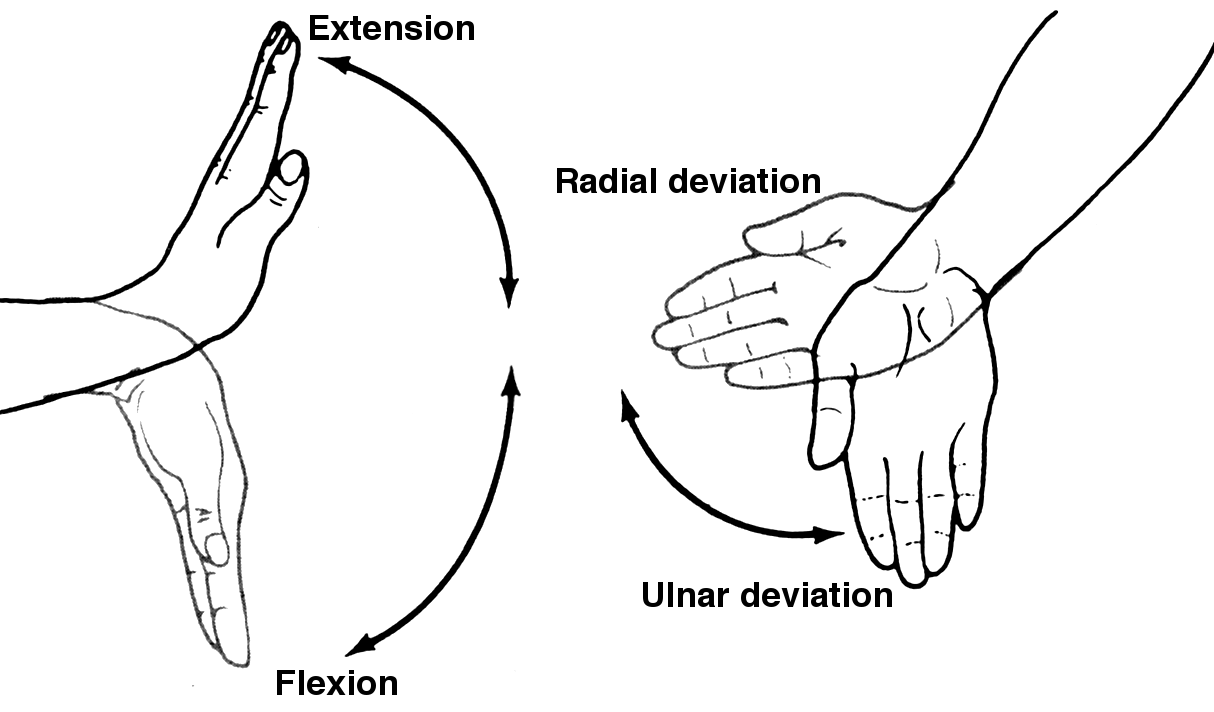
\includegraphics[width=0.4\textwidth]{figures/paperFigures/wristmovement}  %<--but is not needed.
	\caption{Illustration of the two DOF's used in the study (M1: flexion, M2: extension and M3: radial deviation, M4: ulnar deviation)}
	\label{fig:wristmovement}  %<--give the figure a label, so you can reference!
\end{figure}

\begin{figure}[H]
	\centering
	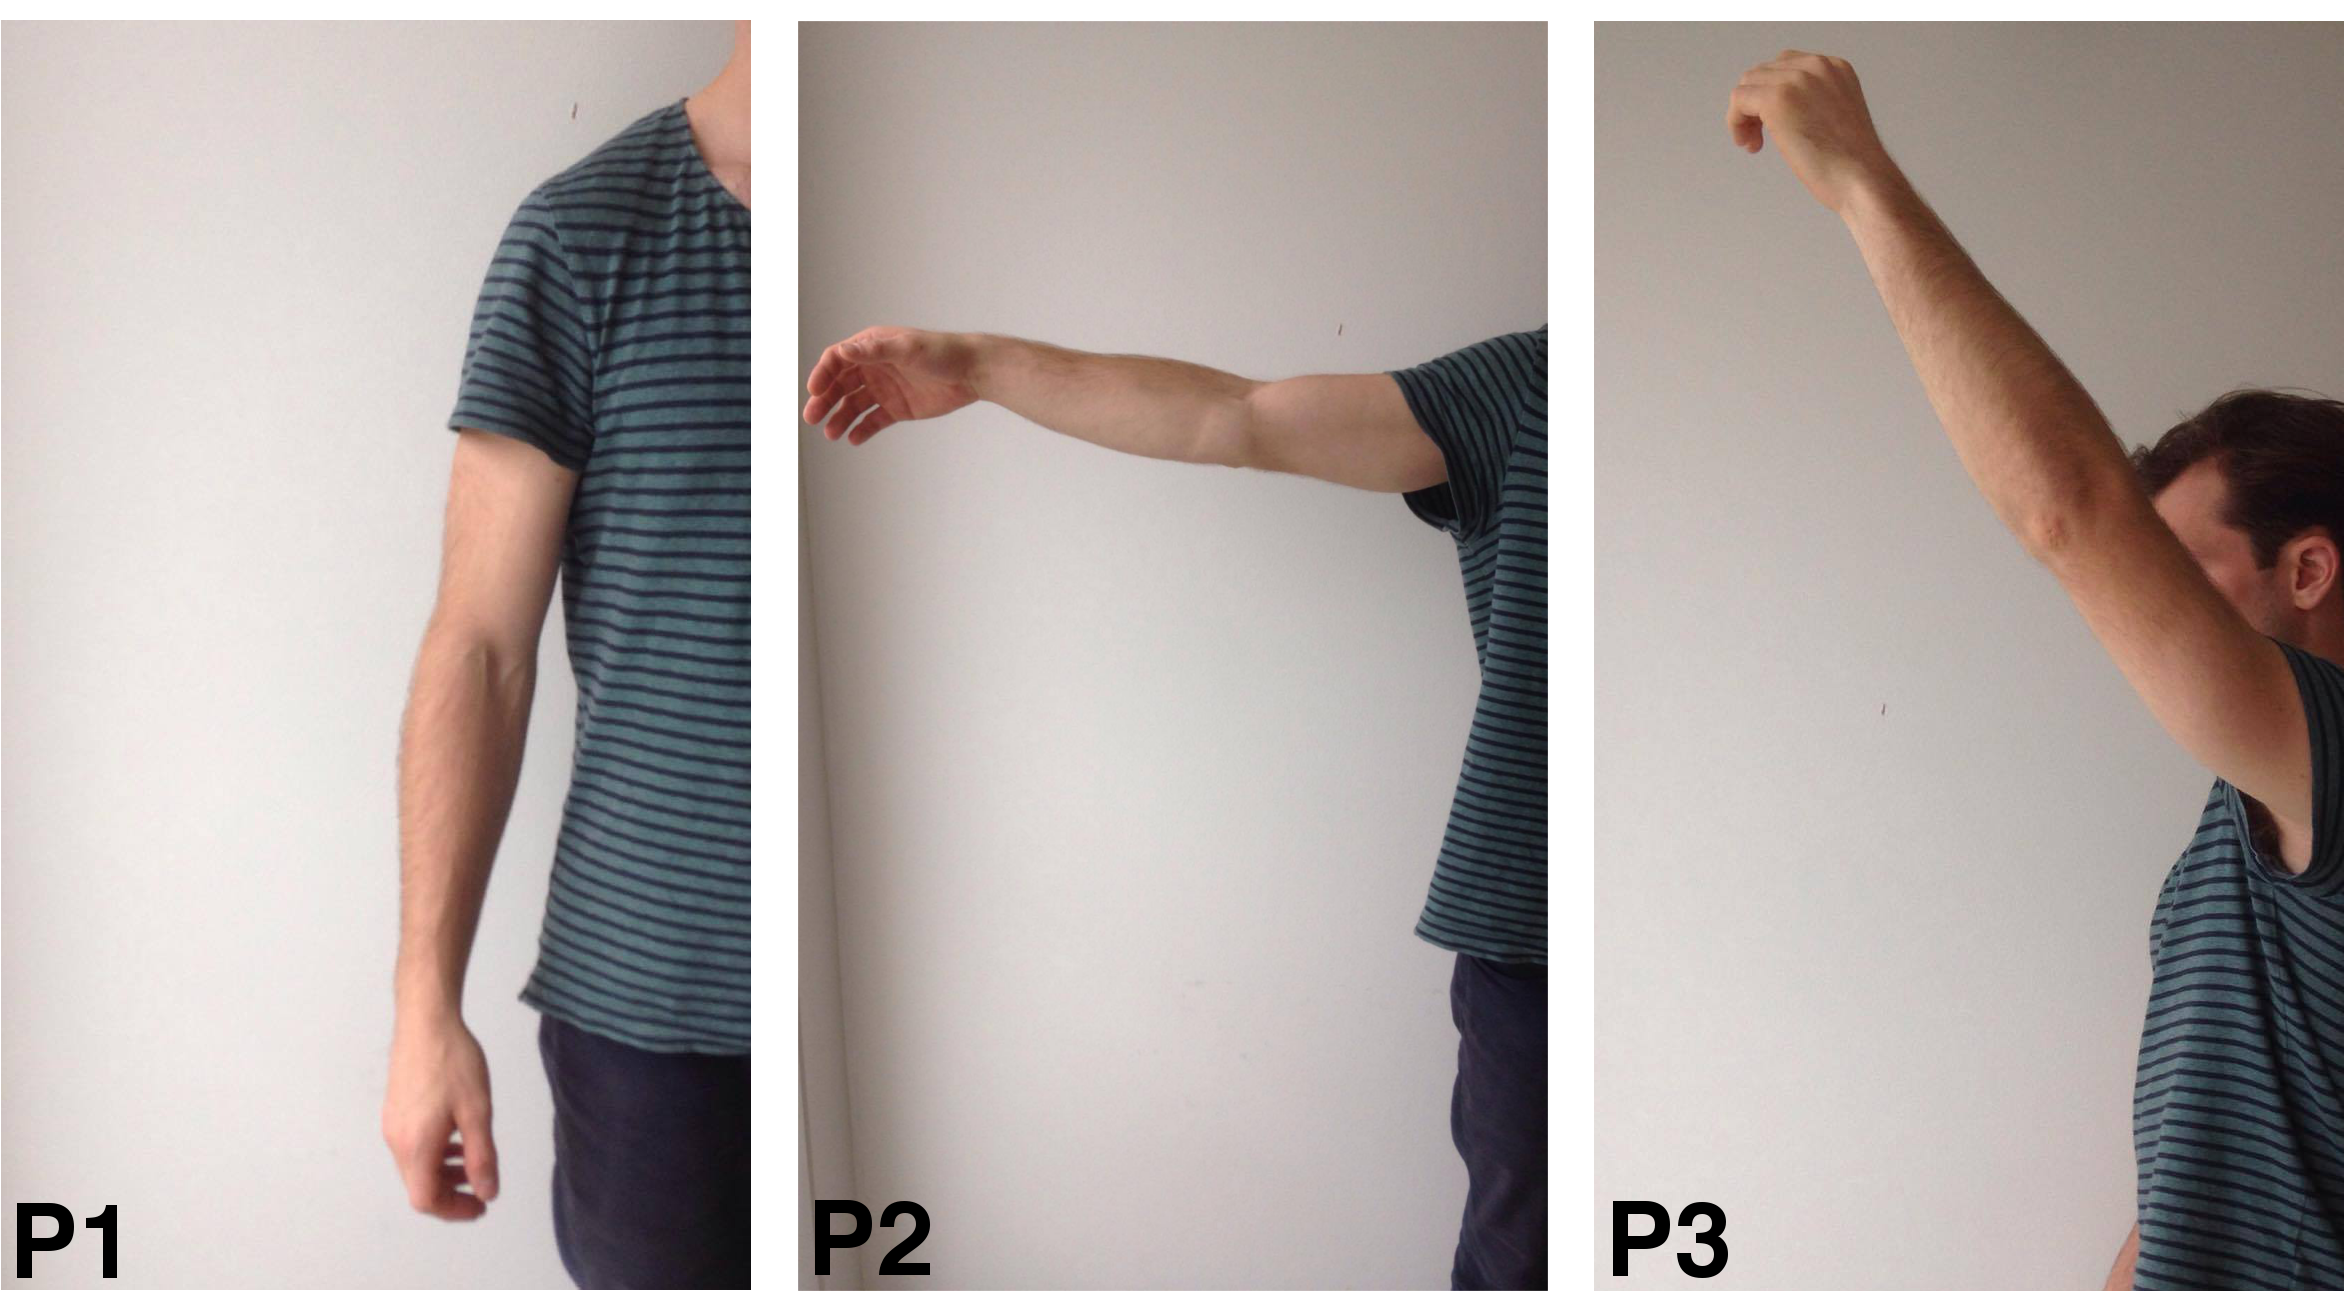
\includegraphics[width=0.4\textwidth]{figures/paperFigures/limb_pos}  %<--but is not needed.
	\caption{Illustration of the limb positions performed. P1: relaxed along the torso, P2: 90 degrees horizontally of the side of torso and P3: 135 degrees vertically in front of the torso}
	\label{fig:limbpositions}  %<--give the figure a label, so you can reference!
\end{figure}

\subsection{Feature extraction}
Features were extracted in a 200 ms window with a 50\% overlap, which is an acceptable segmentation for preserving information of the signal in static contractions \cite{Farfan2010}.
The commonly used Mean Absolute Value (MAV) feature was additionally extracted, and calculated as given by equation \ref{eq:mav}: \cite{Zecca2002} 

\begin{equation} \label{eq:mav}
MAV = \frac{1}{N}\sum\limits_{i=1}^N|x_i|
\end{equation}
where N is the length of the window, and $x_i$ is the EMG signal of $i$ samples.

MAV is directly correlated with change in EMG amplitude. No study has examined whether MAV contains linear properties, but EMG signals has heteroscedastic properties \cite{rasool2012} and the MAV feature might therefore not contain direct linear properties.

In a previous study \cite{hahne2014} it was shown that logarithmizing the variance of EMG the variance linearises, and has yielded robust control of wrist movements in a relaxed limb position when used in linear regression. The Logarithmic Variance (LogVar) was therefore extracted as a feature, and was calculated as given by equation \ref{eq:logvar}:

\begin{equation} \label{eq:logvar}
log(\sigma^2) = log(\frac{\sum\limits_{i=1}^N(x_i - \mu)^2}{N})
\end{equation}
where N expresses the length of the window, $x_i$ is the $i^{th}$ sample of the EMG signal and $\mu$ is the mean.

The Mean Value (MV) was extracted from the accelerometer data, similarly to a previous study \cite{Krasoulis2015} testing the effect of limb position using classification as control scheme. 

The extracted EMG features for the individual wrist movements were examined through a Principal Component Analysis, to evaluate, whether the different movements were distinguishable or new training data should be acquired.

\subsection{Regression model}
As applied in a study by Hwang et al. \cite{hwang2017} to achieve robust performance across variations in limb positions linear regression was used as control scheme. One regressor was trained for each wrist movement for both features; four regressors trained for each feature, and four for each feature where accelerometer data was included. Each regressor was trained based on multivariate linear regression and calculated as given by equation \ref{eq:linearregression}:

\begin{equation} \label{eq:linearregression}
\hat{Y} = \alpha + \beta_1 X_{1} + \beta_2 X_{2} + ... + \beta_i X_{i}
\end{equation}
where $\hat{Y}$ is the estimated value, $X_i$ are the predictors, $\beta_i$ are the regression coefficients in the sampled population, and $\alpha$ is the predicted value of $Y$ at $X_{i} = 0$. $\beta_i$ and $\alpha$ were fitted for each regressor using the extracted feature data for each channel as predictors. The mean of the absolute values of the actual EMG across all channels scaled in relation to the MVC is set as estimator values. The features for all wrist movements in all limb positions were included as predictors in the training of each regressor. However, only the desired wrist movement the regressor was fitted for, was trained with the actual estimated values. The remaining predictors were given 0 as estimated values. This procedure was applied for the regressors to more precisely recognize the performed movement.

\subsection{Offline testing}
The accuracy of the regressors was examined both qualitatively and quantitatively when using both training and test data. A qualitative test was performed by superimposing the regressor output on the actual data. The superimposition illustrated whether the right regressor reacted on the performed movement, and how accurate it responded compared to the actual data. For the quantitative analysis the Root Mean Square Error (RMSE) was calculated to compare through statistical analysis, which feature had the lowest error, and whether the regressors were overfitted when tested with new input data. Furthermore, the accuracy of the regressors trained with inclusion of accelerometer data were compared to the regressors trained only using EMG feature data. The RMSE was calculated as given by equation \ref{eq:rmse}:

\begin{equation} \label{eq:rmse}
RMSE = \sqrt{\frac{\sum\limits_{i=1}^N(y_i - \hat{y_i})^2}{N}}
\end{equation}
where N is the length of the window, $y_i$ is the $i^{th}$ variable of the actual data and $\hat{y_i}$ is the $i^{th}$ output of the regressor.

It was decided, which statistical analysis to apply, through a Kolmogorov-Smirnov test that assesses whether the data populations were normal distributed. An ANOVA test was applied if the data population belonged to a normal distribution, if not a Friedman's test was applied, which is the non-parametric correspondent to an ANOVA test.

\subsection{Online testing}
To investigate the effect of limb position in the regression control scheme an online virtual environment was developed, depicted in figure \ref{fig:targets}

\begin{figure}[H]
	\centering
	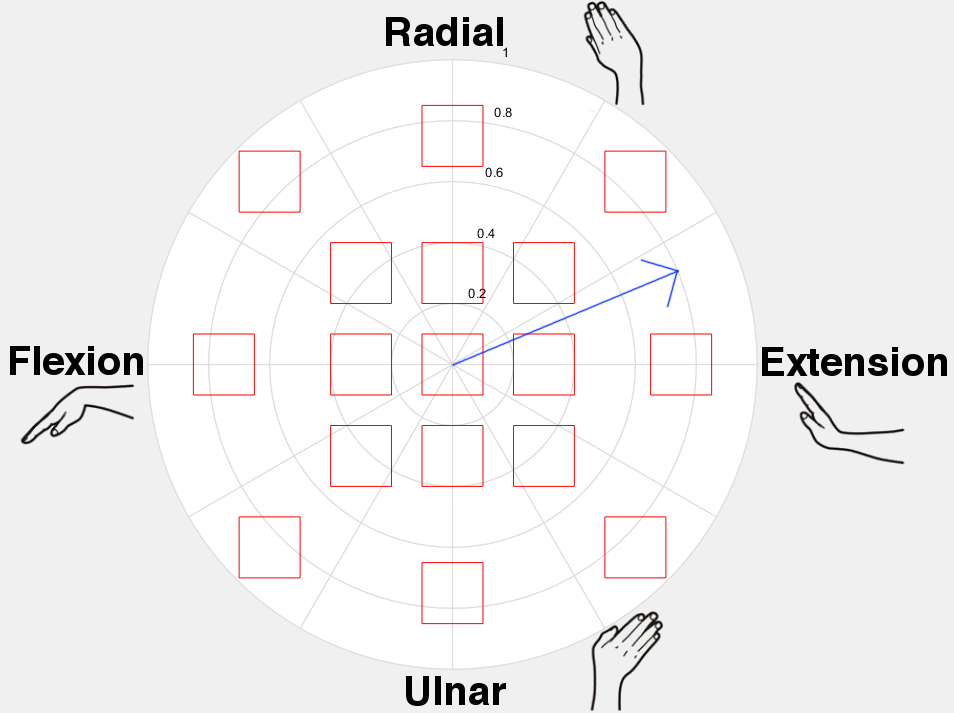
\includegraphics[scale=0.25]{figures/paperFigures/Target}
	\caption{A vector originated from origo depicted the EMG signal, where the length of the vector represented the EMG intensity, and direction was based on the movement performed. The wrist flexion-extension DOF was mapped to the x-axis, and the radial-ulnar deviation DOF was mapped to y-axis. The vector returned to the target located around origo when no contraction was made. For the subject to reach the targets in the diagonals, a simultaneous movement had to be performed. One target was shown at a time. When a target was reached, the vector had to return to the centred target for a new to appear. This gave the subject the same starting point when reaching each outer target. The procedure was performed until all targets had appeared. If a target was not reached within 30 s, it would disappear, and the vector had to return to the centred target.}
	\label{fig:targets}
\end{figure}

The time to complete a target-reaching task of sixteen targets was measured. 12 tests were performed by each subject; one in each limb position for each feature for the regressors trained with and without included accelerometer data. The performance score was calculated as the mean of time per reached target. Time to reach the centred target was not included in the performance score. Performance scores of the online test was compared between the different limb positions of the same feature, between all limb positions of the two features and between performance score obtained when using regressors trained with and without inclusion of accelerometer data. The same comparison was additionally applied for the amount of targets reached. The statistical analysis applied was again based on whether the populations were normal distributed or not. 

\newpage
\clearpage
\end{multicols}

\section{RESULTS}%%%%%%%%%%%%%%%%%%%%%%%%%%%%%%%%%%%%%%%%%%%%%%%%%%%%%%%%%%%%%%%%%%%

\subsection{Offline Results}


\begin{figure}[H]
	\centering
	\subfigure[]{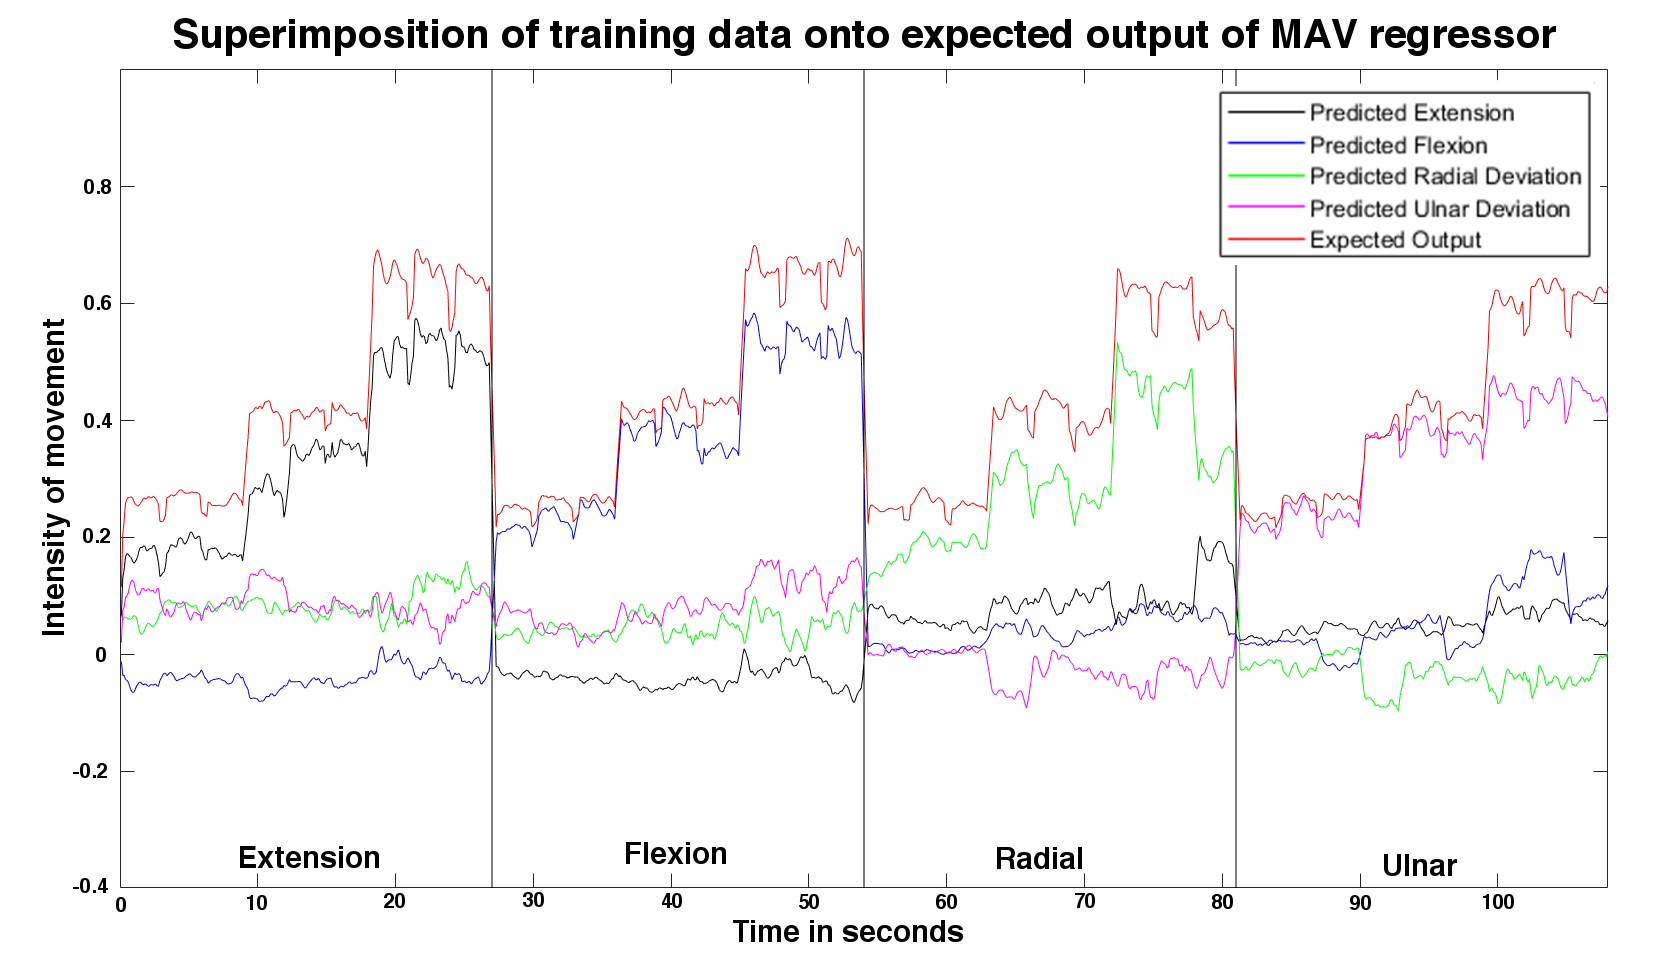
\includegraphics[width=0.95\textwidth]{figures/paperFigures/NewSuperPositionTestDataMAV}}
	\subfigure[]{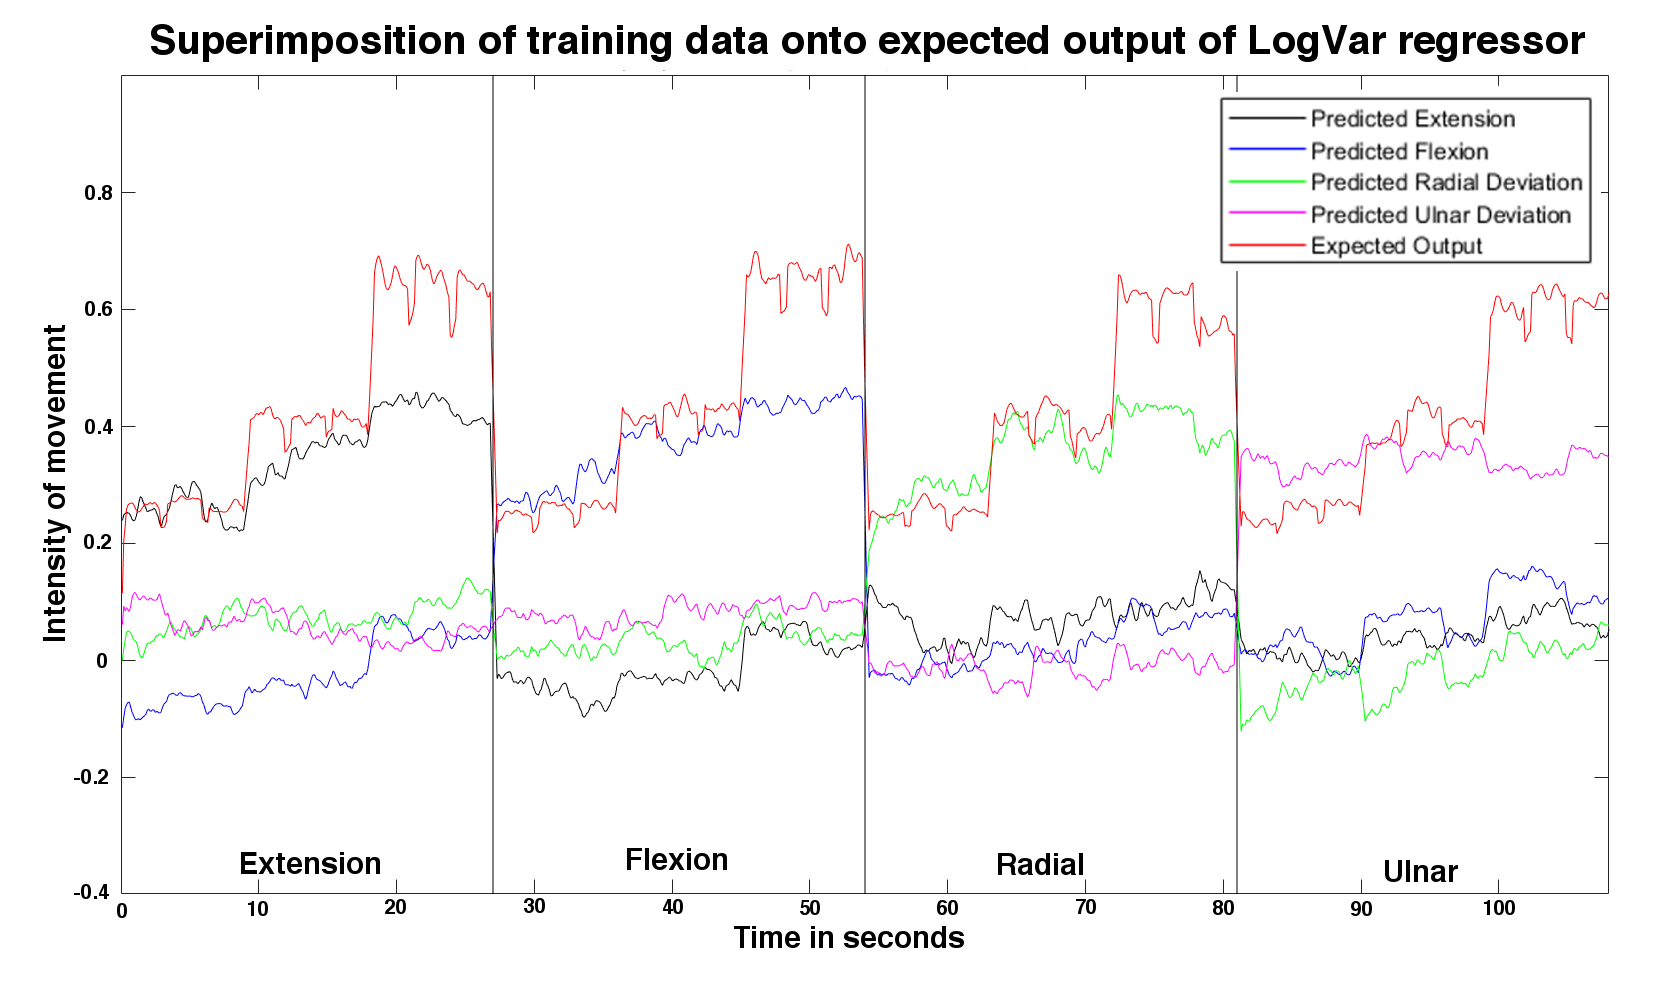
\includegraphics[width=0.95\textwidth]{figures/paperFigures/NewSuperPositionTestDataLogVar}}
	\label{fig:SuperPositionTraining}
	\caption{Plot of the actual data, red plot, superimposed on the output of the regressors trained with the MAV features in (a) LogVar features in (b). The plot is divided into four segments, where each segment shows a different movement performed. Each segment has the same sample size.}
\end{figure}

\begin{multicols}{2}
	

A qualitative examination of the superimposition plots in figure \ref{fig:SuperPositionTraining} shows that each regressor reacts on the movement it is fitted for, and remains inactive when another movement is performed. This accounts for both features. However, both regressors has lower accuracy in the high intensities, especially for the regressors trained with LogVar, which outputs similar values for the 80 \% of MVC contractions as the 50 \% of MVC contractions.
	
	
	\begin{center}
		\scalebox{0.85}{
			\begin{tabular}{l l l} \label{tab:RMSEtrain-test}
				\toprule
				\textbf{Feature} & \textbf{Mean error} & \textbf{Std}\\
				\midrule
%				MAV, Extension & 0.1030 & $\pm 0.0210$ \\
%				MAV, Flexion & 0.1102 & $\pm 0.0296$ \\
%				MAV, Radial Dev. & 0.1206 & $\pm 0.0298$ \\
%				MAV, Ulnar Dev. & 0.1143 & $\pm 0.0334$ \\
				MAV training & 0.1059 & $\pm 0.0306$ \\
				MAV test & 0.1700 & $\pm 0.0759$ \\
%				LogVar, Extension & 0.1157 & $\pm 0.0469$ \\
%				LogVar, Flexion & 0.1102 & $\pm 0.0241$ \\
%				LogVar, Radial Dev. & 0.1142 & $\pm 0.0256$ \\
%				LogVar, Ulnar Dev. & 0.1312 & $\pm 0.0310$ \\
				LogVar training & 0.1178 & $\pm 0.0272$ \\
				LogVar test & 0.1748 & $\pm 0.0563$ \\
				\bottomrule
			\end{tabular}
		}
		\captionof{table}{RMSE for the implemented regression models for both training and test input data.}
	\end{center}
	A Kolmogorov-Smirnov test was applied to all individual data sets in both offline and online test results, and indicated no data set to be normal distributed. Thus, a Friedman's test was applied for all statistical analysis.
	
	Analysing the RMSE of the regression models' response to the training data, it was found that there was a significant difference (p = 0.0044) between MAV and LogVar, where it was shown that LogVar (mean = 0.1178, std = 0.0272) has a higher mean than MAV (mean = 0.1059, std = 0.0306), as seen in table \ref{tab:RMSEtrain-test}. 
	
	
%	\begin{center}
%		\scalebox{0.85}{
%			\begin{tabular}{l l l}
%				\toprule
%				\textbf{Feature} & \textbf{Mean error} & \textbf{Std}\\
%				\midrule
%%				MAV, Extension & 0.1646 & $\pm 0.0753$ \\
%%				MAV, Flexion & 0.1391 & $\pm 0.0841$ \\
%%				MAV, Radial Dev. & 0.2018 & $\pm 0.0424$ \\
%%				MAV, Ulnar Dev. & 0.1743 & $\pm 0.0905$ \\
%				MAV overall & 0.1700 & $\pm 0.0759$ \\
%%				LogVar, Extension & 0.1552 & $\pm 0.0514$ \\
%%				LogVar, Flexion & 0.1680 & $\pm 0.0508$ \\
%%				LogVar, Radial Dev. & 0.1681 & $\pm 0.0540$ \\
%%				LogVar, Ulnar Dev. & 0.2078 & $\pm 0.0621$ \\
%				LogVar overall & 0.1748 & $\pm 0.0563$ \\
%				\bottomrule
%			\end{tabular}
%		}
%		\captionof{table}{RMSE for test data input for the regression models}
%	\end{center}
	
	\begin{center}
		\scalebox{0.85}{
			\begin{tabular}{l l} \label{tab:RMSEp-values}
				\toprule
				\textbf{Compared features} & \textbf{P-Value}\\
				\midrule
				LogVar, MAV & 0.0044 \\
				LogVar test data, MAV test data & 0.1138 \\
				LogVar test data, LogVar & 0.0001 \\
				MAV test data, MAV & 0.000002 \\
				\bottomrule
			\end{tabular}
		}
		\captionof{table}{P-Values for comparison of the features.}
	\end{center}
	
	A significant difference was found (p = 0.0001) between the RMSE for test data (mean = 0.1748, std = 0.0563) and training data (mean = 0.1178, std = 0.0272) for LogVar, as shown in table \ref{tab:RMSEp-values}. A significant difference (p = 0.000002) was also found for the test data (mean = 0.1700, std = 0.0759) and training data (mean = 0.1059, std = 0.0306) for the MAV based regression models. No significant difference (p = 0.1138) was found between MAV (mean = 0.1700, std = 0.0759) and LogVar (mean = 0.1748, std = 0.0563) regression models with test data.
	
	\subsection{Online Results}

\begin{figure}[H]
	\centering
	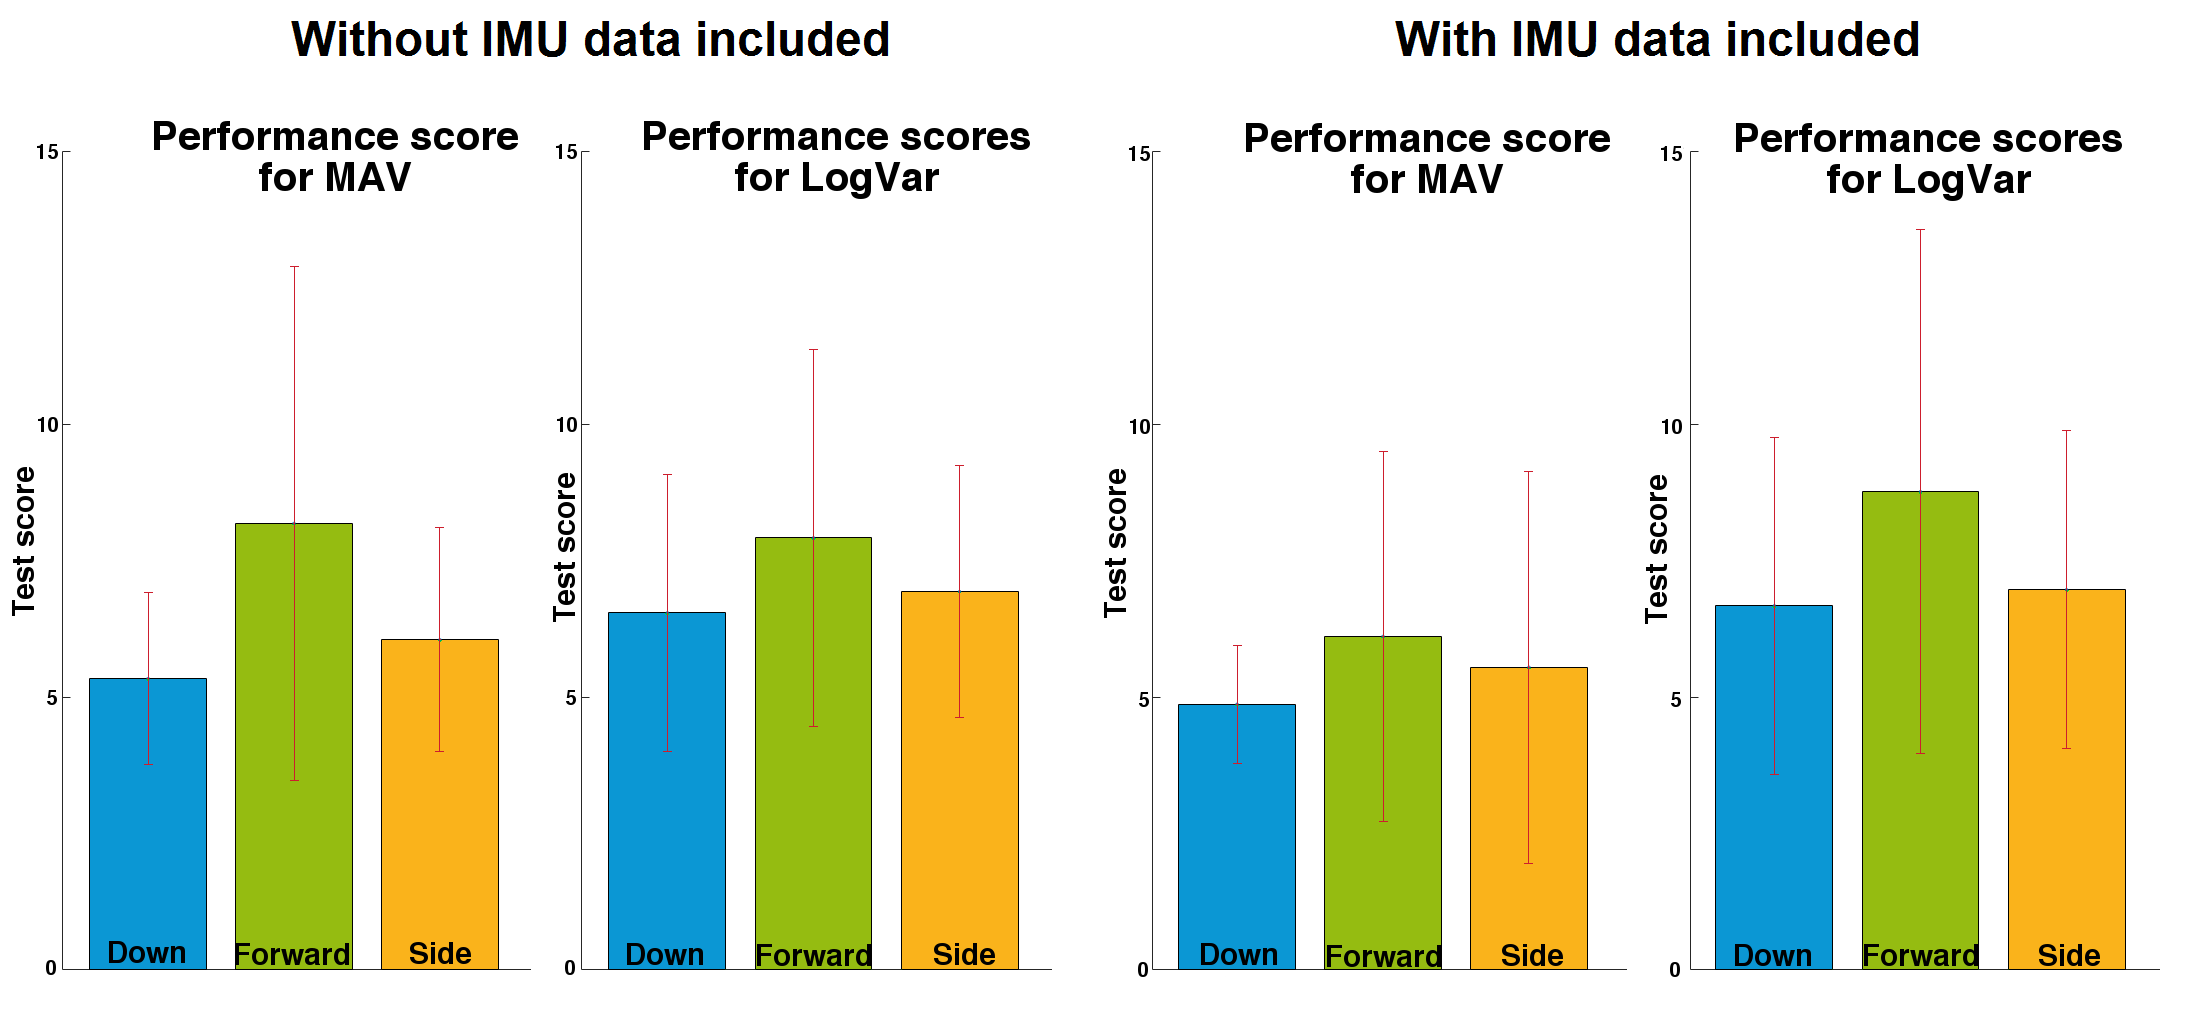
\includegraphics[width=1\textwidth]{figures/paperFigures/GotItTimeCol}  %<--but is not needed.
	\caption{Bar chart of the performance scores for MAV and LogVar features without (figure A) and with inclusion of IMU data (figure B).}
	\label{fig:GotItTimeCol}
\end{figure}
	
\begin{figure}[H]
	\centering
	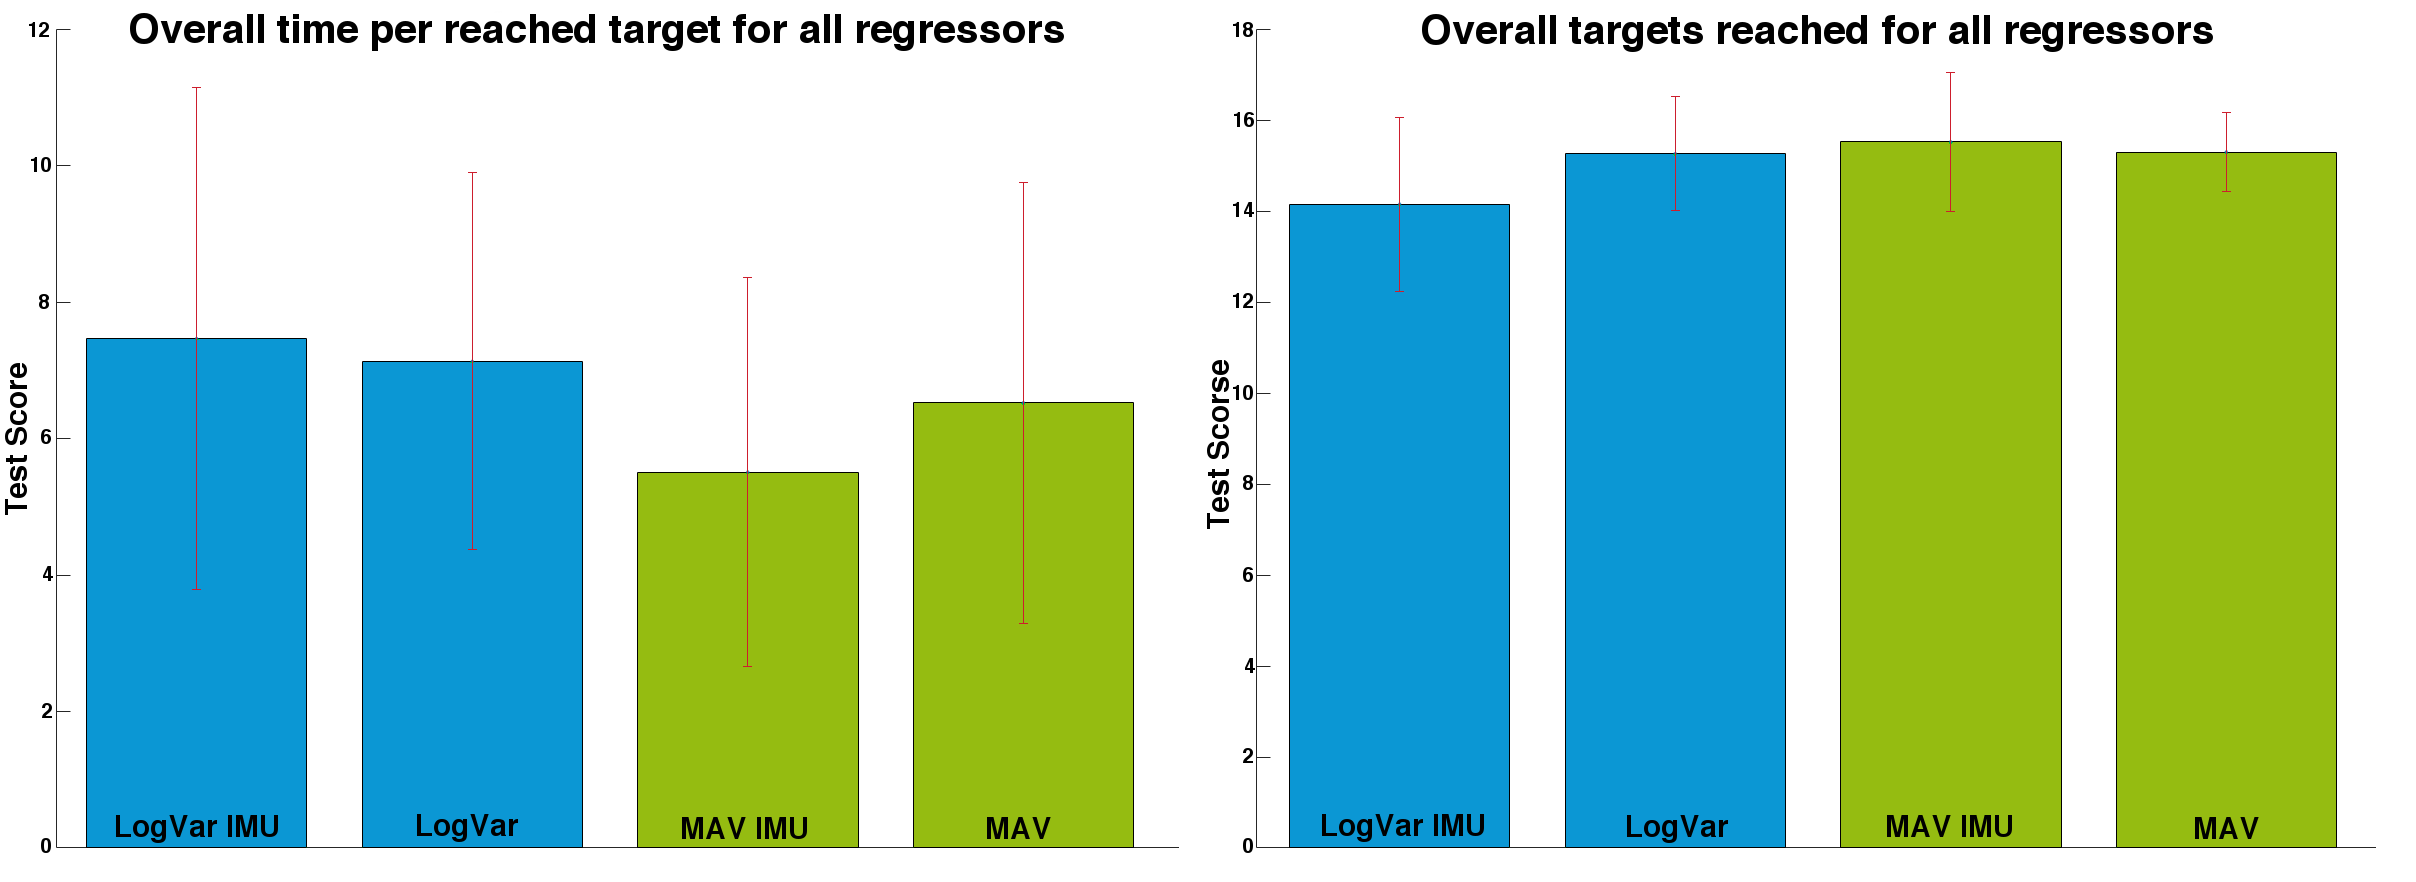
\includegraphics[width=1\textwidth]{figures/paperFigures/allRegressorBarzTimeScoreForTargetTestCol}  %<--but is not needed.
	\caption{Figure A shows the bar chart of the overall performance scores for MAV and LogVar features without and with inclusion of IMU data. Figure B shows the overall number of targets reached for MAV and LogVar features without and with inclusion of IMU data.}
	\label{fig:TargetScoresTargetsCol}  %<--give the figure a label, so you can reference!
\end{figure}
	
%\newpage

		\begin{center}
			\scalebox{0.85}{
			\begin{tabular}{l l l}
				\toprule
				\textbf{Position, feature} & \textbf{PS} & \textbf{Std}\\
				\midrule
				Down, MAV & 5.3377 & $\pm 1.5696$ \\
				Forward, MAV & 8.1791 & $\pm 4.7145$ \\
				Side, MAV & 6.0490 & $\pm 2.0490$ \\
				Down, LogVar & 6.5404 & $\pm 2.5315$ \\
				Forward, LogVar & 7.9123 & $\pm 3.4572$ \\
				Side, LogVar & 6.9325 & $\pm 2.3036$ \\
				\bottomrule
			\end{tabular}
		}
			\captionof{table}{Performance score (PS) for the different limb positions for MAV and LogVar regressors.}
		\end{center}

\begin{center}
	\scalebox{0.85}{
		\begin{tabular}{l l}
			\toprule
			\textbf{Feature} & \textbf{P-Value}\\
			\toprule
			MAV & 0.0319 \\
			LogVar & 0.4594 \\
			\toprule
		\end{tabular}
	}
	\captionof{table}{P-Values for comparison of the scores across different limb positions with MAV and LogVar.}
\end{center}

		
	
	When comparing the score for different limb positions, no significant difference was found for either MAV (p = 0.8948) or LogVar (p = 0.2359).
	
		\begin{center}
			\scalebox{0.85}{
			\begin{tabular}{l l l}
				\hline
				\textbf{Position, feature} & \textbf{TR} & \textbf{Std}\\
				\hline
				Down, MAV & 15.5556 & $\pm 0.7265$ \\
				Forward, MAV & 15.1111 & $\pm 1.0541$ \\
				Side, MAV & 15.2222 & $\pm 0.8333$ \\
				Down, LogVar & 15.4444 & $\pm 0.7265$ \\
				Forward, LogVar & 15 & $\pm 1.8020$ \\
				Side, LogVar & 15.3333 & $\pm 1.1180$ \\
				\hline
			\end{tabular}
		}
			\captionof{table}{Targets reached (TR) in the target reaching test with the MAV and LogVar regressors.}
		\end{center}
	
	
		\begin{center}
			\scalebox{0.85}{
			\begin{tabular}{l l}
				\toprule
				\textbf{Feature} & \textbf{P-Value}\\
				\midrule
				MAV & 0.2285 \\
				LogVar & 0.7788 \\
				\bottomrule
			\end{tabular}
		}
			\captionof{table}{P-Values for comparison of the number of reached targets across different limb positions with MAV and LogVar.}
		\end{center}
	
	It was shown that there is no significant difference (p = 0.2285) between the number of targets reached in the different positions for MAV, where the limb pointed forward yielded worst results (mean = 15.1111, std = 1.0541). No significant difference (p = 0.7788) was found between the limb positions for LogVar.
	
	
	
		\begin{center}
			\scalebox{0.85}{
			\begin{tabular}{l l l}
				\toprule
				\textbf{Position,feature} & \textbf{PS} & \textbf{Std}\\
				\midrule
				Down, MAV & 4.8661 & $\pm 1.0839$ \\
				Forward, MAV & 6.1094 & $\pm 3.3852$ \\
				Side, MAV & 5.5442 & $\pm 3.5847$ \\
				Down, LogVar & 6.6691 & $\pm 3.0798$ \\
				Forward, LogVar & 8.7595 & $\pm 4.7969$ \\
				Side, LogVar & 6.9652 & $\pm 2.9144$ \\
				\bottomrule
			\end{tabular}
		}
			\captionof{table}{Performance score (PS) for the different limb positions for MAV and LogVar regressors with IMU included.}
		\end{center}
	
		\begin{center}
			\scalebox{0.85}{
				\begin{tabular}{l l}
					\toprule
					\textbf{Feature} & \textbf{P-Value}\\
					\midrule
					MAV & 0.8948 \\
					LogVar & 0.2359 \\
					\bottomrule
				\end{tabular}
			}
			\captionof{table}{P-Values for comparison of the performance scores across different limb positions with MAV and LogVar regressors including IMU data.}
		\end{center}
		
	
	No significant difference (p = 0.8948) was found between the performance scores across different limb positions for MAV with IMU included. No significant difference (p = 0.2359) was found between limb positions for the LogVar regression model with IMU data included.
	
	
		\begin{center}
			\scalebox{0.85}{
			\begin{tabular}{l l l}
				\toprule
				\textbf{Position,feature} & \textbf{TR} & \textbf{Std}\\
				\midrule
				Down, MAV & 15.8889 & $\pm 0.3333$ \\
				Forward, MAV & 15.1111 & $\pm 2.3154$ \\
				Side, MAV & 15.5556 & $\pm 1.3333$ \\
				Down, LogVar & 14.7778 & $\pm 1.7159$ \\
				Forward, LogVar & 13.5556 & $\pm 2.1858$ \\
				Side, LogVar & 14.1111 & $\pm 1.8333$ \\
				\bottomrule
			\end{tabular}
		}
			\captionof{table}{Targets reached (TR) in the target reaching test with the MAV and LogVar regressors with inclusion of IMU data.}
		\end{center}
		
		\begin{center}
			\scalebox{0.85}{
			\begin{tabular}{l l}
				\toprule
				\textbf{Compared Features} & \textbf{P-Value}\\
				\midrule
				MAV & 0.4966 \\
				LogVar & 0.0957 \\
				\bottomrule
			\end{tabular}
		}
			\captionof{table}{P-Values for comparison of the number of targets reached in different limb positions with MAV and LogVar with IMU data included.}
		\end{center}
	
	There was no significant difference found for the MAV regressor with IMU data included (p = 0.4966). The number of targets reached in different limb positions was not proven significantly different (p = 0.0957) for the LogVar feature with IMU data included, but had a lower mean of number of reached targets compared to MAV as seen in table \ref{tab:averageNoTR}.

		\begin{center}
			\scalebox{0.85}{
			\begin{tabular}{l l l}
				\toprule
				\textbf{Feature} & \textbf{Mean PS} & \textbf{Std}\\
				\midrule
				MAV & 6.5219 & $\pm 3.2253$ \\
				MAV w. IMU & 5.5066 & $\pm 2.8477$ \\
				LogVar & 7.1284 & $\pm 2.7619$ \\
				LogVar w. IMU & 7.4646 & $\pm 3.6740$ \\
				\bottomrule
			\end{tabular}
		}
			\captionof{table}{Average performance score (PS) of the target reaching test for the four regressor designs.}
		\end{center}

	

		\begin{center}
			\scalebox{0.85}{
			\begin{tabular}{l l}
				\toprule
				\textbf{Compared features} & \textbf{P-Value}\\
				\midrule
				LogVar, MAV & 0.0833 \\
				LogVar w/ IMU, MAV w/ IMU & 0.5637 \\
				MAV, MAV w/ IMU & 0.1779 \\
				LogVar, LogVar w/ IMU & 0.5637 \\
				\bottomrule
			\end{tabular}
		}
			\captionof{table}{P-Values for comparison of the overall scores of the target reaching tests.}
		\end{center}

	
	A significant difference (p = 0.5637) could not be proven between the scores of the target reaching test for LogVar with IMU data and MAV with IMU data. There was no significant difference (p = 0.0833) between the score of LogVar without IMU data and MAV without IMU data. It was also found that there is no significant difference between regression models with and without IMU data for both MAV (p = 0.1179) and LogVar (p = 0.5637).	
	
	
		\begin{center}
			\scalebox{0.85}{
			\begin{tabular}{l l l} \label{tab:averageNoTR}
				\toprule
				\textbf{Feature} & \textbf{Mean TR} & \textbf{Std}\\
				\midrule
				MAV & 15.2963 & $\pm 0.8689$ \\
				MAV w/ IMU & 15.5185 & $\pm 1.5285$ \\
				LogVar & 15.2593 & $\pm 1.2586$ \\
				LogVar w/ IMU & 14.1481 & $\pm 1.9156$ \\
				\bottomrule
			\end{tabular}
		}
			\captionof{table}{Average number of targets reached (TR) in the target reaching test for the four regressor designs.}
		\end{center}
	
	
		\begin{center}
			\scalebox{0.85}{
			\begin{tabular}{l l}
				\toprule
				\textbf{Compared Features} & \textbf{P-Value}\\
				\midrule
				LogVar, MAV & 1 \\
				LogVar w/ IMU, MAV w/ IMU & 0.0017 \\
				MAV, MAV w/ IMU & 0.0124 \\
				LogVar, LogVar w/ IMU & 0.0016 \\
				\bottomrule
			\end{tabular}
		}
			\captionof{table}{P-Values for comparison of number of targets reached in the target reaching tests.}
		\end{center}
	
	A significant difference (p = 0.0017) was found between targets reached when IMU was included, where LogVar (mean = 14.1481, std = 1.9156) was proven worse than MAV (mean = 15.5185, std = 1.5285). There was a significant difference (p = 0.0016) between LogVar with (mean = 14.1481, std = 1.9156) and without (mean = 15.2593, std = 1.2586) IMU data. The same significant difference (p = 0.0124) between MAV with (mean = 15.5185, std = 1.5285) and without (mean = 15.2963, std = 0.8689) IMU data. There was no difference (p = 1) between targets reached with LogVar and MAV when IMU was not included.
	
\section{DISCUSSION}%%%%%%%%%%%%%%%%%%%%%%%%%%%%%%%%%%%%%%%%%%%%%%%%%%%%%%%%%%%%%%%%
	
%		%discussion points
The present paper had as porpuose to study the performance of linear regression methods for myoelectric prostheses control taking in acount the limb position effect. Along the process different aspects have been exposed that are important to mention.\\
%subdivide in sections??
%Potential outliers were discoverd during this study. Even though the final results present that is possible to achieve simultaneous and proportional control using Myo armband, it had been shown that the sampling rate of this device could affect the acquisition of sEMG data. This could be due to the fact that sEMG signals  rate is between 10-500Hz, however the sampling rate of the Myoarmband is 200Hz, which casuses important information in raw data to be eliminated.
%Based on prevoius studies two different features were extracted in order to tran the regressors MAV and LogVar.
%A study by Hanhe \cite{hanhe2014} et al. showed that LogVar presented linear properties and outperformed the other different features extracted for that particular research. However the obtained results in our study illustrates that MAV performance outperformed the LogVar results. 
%Futhermore online results were not siginificant different depending on the limb position as other studies had shown for classification control scheme. This findings agree with a recently published study by Hwang et al. \cite{Hwang2017}. In their study different limb position were tested using Root Mean Square (RMS) as feature to train the regressors.
%During the results examination it was found that there is no correlation between the offline and online results. On the one hand the offline outcomes illustrates overfitting of the regression models. On the other hand the online test yielded robust control of the wrist movements performanced in the three different limb positions. This could be owing to the subjects$'$ ability to compensate for a poorer fitting model when visual feedback is provided.
%It have been proved that is possible to achieve simultaneous and proportional control in myoelectric prosthesis using linear regression techniques. 
%\begin{itemize}
	%\item inclusion of more subjects
%	\item sample rate of the myo armband - exclusion of test subjects
	%\item even though LogVar shows linearity in a previous study, it does not perform better in linear regression than a presumably non-linear feature
	%\item Both features does not show significant difference in control in different limb positions
%	\item Whatever the inclusion of IMU shows 
	
%	\item It is possible to use regression as control method to yield no significantly different performance in variations of limb positions
	%\item Use other regression methods and other features to analyse if it will result in better performance
	%\item why does the inclusion of IMU improve the performance
%	\item No connection between offline and online tests, which also is shown in previous studies
%	\item reasonable control can be archived when donning/doffing(we train the regressors with data, take of the myo armband, and do the testing with the myo armband placed slightly elsewhere)
	
%\end{itemize}
	\subsection{Offline and online training}
	Offline and online training was done for both MAV and LogVar without IMU data included, with a significant difference between the two features when testing with training data (p = 0.0044) but no difference when testing with new data (p = 0.1138). Overall it was found that there were no apparent correlation between offline and online testing. This could be caused by the subjects ability to adjust to a poor fitted model when given the visual feedback while performing the target test. This finding corresponds to the findings in other studies \cite{jiang2010}.
	
	\subsection{Comparison of features}
	In the results it was found that there was no significant difference between the performance of LogVar and MAV when it comes to the scores for the target test both with (p = 0.5637) and without (p = 0.0833) IMU data included. Based on previous studies showing LogVar as a feature with linear properties, it would be expected that this feature would perform better in a linear regression model, than a feature which to the authors knowledge has not been proven to be linear. On the contrary it was shown that a significantly higher number of targets was reached with a linear regression models based on the MAV feature with IMU included, compared to the LogVar regression model with IMU included (p = 0.0017). When IMU data wasn't included, there was no difference between the number of targets reached in the test (p = 1).
	
	Further studies within this field should consider examining other features, while studying the effect of combining several features in order to yield better performance independent of the limb position.
	
	\subsection{Inclusion of IMU data}
	The IMU data included in this study was based on a single accelerometer, where it was expected that the Myo band would give a similar output as long as the subjects were performing both training and testing from the same starting position. Inclusion of the IMU data was shown to yield the same results when it comes to the test score, with no significant difference for either MAV (p = 0.1779) or LogVar (p = 0.5637) when comparing regression models build with and without accelerometer inputs. It was found that the inclusion of the IMU data yielded significantly worse results for the LogVar regression model (p = 0.0016), while it led to a significant improvement of the MAV regression model (p = 0.0124) when examining the number of reached targets. The inclusion of IMU data could be a subject of further investigation, as the results might be improved by implementing a system capable of measuring the angles of the joints, in order to create a more versatile and usable regression model outside the clinical environment.  
	
	\subsection{Stability in limb positions}
	When excluding IMU data, there was no significant difference between the target score for either LogVar (p = 0.2359) or MAV (p = 0.8948) in the different limb positions, while there was a difference between the number of reached targets for MAV (0.0212) but no difference for LogVar (p = 0.4220). This outcome shows that both MAV and LogVar yields rather stable performance in different limb positions when used to create linear regression based control schemes.
	
	When including IMU data the MAV based regression model was shown to have a significant difference between the score of different limb positions (p = 0.0319), while LogVar did not show any difference (p = 0.4594). While the time taken to reach targets were shown to be different depending on limb positions when using MAV, the number of targets reached was improved, so that the number of reached targets with MAV were not shown to be significantly different (p = 0.2957). The LogVar feature based regression models were shown to have a difference between reached targets when using IMU data (p = 0.0037).
	
	Overall the LogVar regression models were observed as being the most unstable in the different limb positions when looking at the test subjects performance in the target test. This might be a result of the LogVar feature being based on the change of the signal, as this could lead to problems with crosstalk when the arm is not in a relaxed state. The MAV was observed as being more stable, with the subjects being able to create more controlled movements as well as having the possibility to adjust the position of the arrow when trying to get back to the middle of the test GUI. Based on the findings of this study, it would be recommended to examine features based on the amplitude rather than the variance in future studies within this area.
	
	\subsection{Limitations of the study}
	This study was based on data from 12 test subjects, where three had to be excluded. One subject was excluded due to misunderstanding the given instructions and thereby creating an unusable set of training and test data, which limited the control of the regression models giving him a mean score above 25 seconds per target and average number of reached targets below 10 for all tests.
	
	Two other subjects were excluded as the recorded intensities were not high enough to differ between the baseline and the intended movement. This caused the regression models to interpret the baseline in the target test as movements being performed at between 30\% and 70\% of the MVC.
	
	To improve the validity of the study more test subjects should be included in further studies within this field. Subjects with transradial amputations should also be taken into consideration if the regression based control schemes were to be considered for future use in myoelectric prosthetic devices. 
	
	Using the Myo band for data acquisition led to certain limitations in the sample rate, as the device is only capable of recording signals between 0 and 200Hz. This leads to the final signal being recorded between 0 and 100Hz, where everything above 100Hz is affected by aliasing. Along with frequency limitations, the Myo band restricted the number and placement of electrodes to eight channels placed at the same distance from the elbow, where it might be possible to yield better results with a different electrode placement and number. Further studies should implement regular EMG electrodes in order to obtain a more usable and clear signal, that represents the entire frequency band of EMG signals.
	
	
%	\begin{table}[h]
%		\caption{An Example of a Table}
%		\label{table_example}
%		\begin{center}
%			\begin{tabular}{|c||c|}
%				\hline
%				One & Two\\
%				\hline
%				Three & Four\\
%				\hline
%			\end{tabular}
%		\end{center}
%	\end{table}
	


	
	
	%Figure Labels: Use 8 point Times New Roman for Figure labels. Use words rather than symbols or abbreviations when writing Figure axis labels to avoid confusing the reader. As an example, write the quantity ÒMagnetizationÓ, or ÒMagnetization, MÓ, not just ÒMÓ. If including units in the label, present them within parentheses. Do not label axes only with units. In the example, write ÒMagnetization (A/m)Ó or ÒMagnetization {A[m(1)]}Ó, not just ÒA/mÓ. Do not label axes with a ratio of quantities and units. For example, write ÒTemperature (K)Ó, not ÒTemperature/K.Ó
\textbf{Comparison of features.}
The online results indicated no significant difference between LogVar and MAV in the performance scores both with (p = 0.5637) and without (p = 0.0833) IMU data included. Based on a study \cite{hahne2014} showing LogVar as a feature with linear properties, it would be expected that this feature would perform better in a linear regression model, than a feature which to the authors knowledge has not been proven to be linear. On the contrary it was shown that a significantly higher number of targets was reached with a linear regression models based on the MAV feature with IMU included, compared to the LogVar regression model with IMU included (p = 0.0017). When IMU data was not included, there was no difference between the number of targets reached in the test (p = 1).

Further studies within this field should consider examining other features and studying the effect of combining several features in order to further improve performance independent of the limb position.

\textbf{Inclusion of IMU data.}
The IMU data included in this study was based on a single accelerometer, where it was expected that the Myo armband would give a similar output as long as the subjects were performing both training and testing from the same starting position. Inclusion of the IMU data was shown to yield the same results in the online performance scores, with no significant difference for either MAV (p = 0.1779) or LogVar (p = 0.5637) when comparing regression models trained with and without accelerometer inputs. Inclusion of the IMU data yielded significantly poorer results for the LogVar regression model (p = 0.0016), while it led to a significant improvement of the MAV regression model (p = 0.0124) when examining the number of reached targets. The inclusion of IMU data could be a subject of further investigation, as the results might be improved by implementing a system capable of measuring the angles of the joints, in order to create a more versatile and usable regression model outside the clinical environment. Including IMU data could additionally be used to select specific regression models, if a system was build with models fitted for each limb position instead of the same regressors for all positions. 

\textbf{Stability in limb positions.}
Without IMU data there was no significant difference between the performance score for LogVar (mean = 7.1284, p = 0.4594)  in the different limb positions, but for MAV (mean = 6.5219, p = 0.0391) there was, while there was no significant difference between the number of reached targets for MAV (mean = 15.2963, 0.2285) or LogVar (mean = 15.2593, p = 0.7788). This outcome shows that both MAV and LogVar yields stable performance in different limb positions in a linear regression-based control scheme. This finding agrees with Hwang et al. \cite{Hwang2017}, who equivalently found stable online performance across limb positions in a linear regression-based control scheme applying RMS as feature.

When including IMU data the MAV based regression model was shown to have no significant difference in scores across limb positions (mean = 5.5066, p = 0.8948). Same results were yielded for LogVar (mean = 7.4646, p = 0.2359).  There was no significant difference in the amount of targets reached for the MAV trained regressors (mean = 15.5185, p = 0.4966) and the LogVar trained regressors (mean = 14.1481, p = 0.0957). 

Overall the LogVar regression models were observed as being the most unstable in the different limb positions when examining the test subjects performance in the target-reaching test. This is due to the lower mean performance scores and number of reached targets both when trained with and without IMU data. This might be a result of the LogVar feature being based on the change of the signal, as this could lead to problems with crosstalk, when the arm is not in a relaxed state. MAV was observed as being more stable, with the subjects being able to create more smooth movements as well as being able to controllably return to the resting position. Based on the findings of this study, it would be recommended to examine features based on the amplitude rather than the variance in future studies within this area.

\textbf{Offline vs. online training.}
Offline testing was only done for MAV and LogVar without IMU data included. A significant difference between the two features when testing with training data (p = 0.0044) was archived in the offline test, but no significant difference when testing with new data (p = 0.1138). Comparing RMSE of LogVar with training data and RMSE of LogVar with new data there was a significant difference (P = 0.0001), where RMSE of the test with new data has the higher mean. Same results were yielded for the MAV trained regressors (P = 0.000005). This indicates that the regression models were overfitted when exposed to new data. The online results yielded robost control across all limb positions, and therefore no apparent correlation between offline and online testing. This could be caused by the subjects ability to adjust to a poor fitted model when given visual feedback while performing the target-reaching test. This observation corresponds to findings in another study \cite{jiang2010}.

\textbf{Limitations of the study.}
This study was based on data from 12 test subjects, where three had to be excluded. One subject was excluded due to misunderstanding the given instructions and thereby creating an unusable set of training and test data. This limited the control of the regression models giving the subject a mean score above 25 s per target reached and average number of reached targets below 10 for all tests.

Two other subjects were excluded as the recorded intensities were not high enough to differ between the baseline and the higher EMG intensity. This caused the regression models to interpret the baseline in the target-reaching test as movements being performed at between 30\% and 70\% of the MVC. 

To improve the validity of the findings more test subjects should be included in future studies within this field. Subjects with transradial amputations should also be taken into consideration if regression based control schemes were to be considered for future use in myoelectric prosthetic devices. 

Using the Myo armband for data acquisition limited the sampling rate to 200 Hz. Only the 0-100 Hz spectrum of the EMG was represented correctly, where frequencies above 100 Hz was affected by aliasing. Along with frequency representation limitations, the Myo armband restricted the number and placement of electrodes to eight channels placed at the same distance distal to the elbow joint, where it might be possible to yield better results with a different electrode placement and number of channels. Further studies should implement conventional EMG electrodes and an ADC with a sufficient sample rate, enabling the entire frequency band of EMG signals to be acquired correctly.		
	
\section{CONCLUSIONS}%%%%%%%%%%%%%%%%%%%%%%%%%%%%%%%%%%%%%%%%%%%%%%%%%%%%%%%%%%%%%%%
	
% 		Linear regression methods were applied for the two different features extracted. We compared both performance, training the regressor with EMG data as well as a combination of EMG data and IMU data.
	
	\addtolength{\textheight}{-12cm}   % This command serves to balance the column lengths
	% on the last page of the document manually. It shortens
	% the textheight of the last page by a suitable amount.
	% This command does not take effect until the next page
	% so it should come on the page before the last. Make
	% sure that you do not shorten the textheight too much.
In conclusion linear regression can be implemented as control scheme in myoelectric prosthetic control to yield performance with no significant difference across variations of limb position. This is opposed to previous studies using classification as control scheme.
 		
	
	%%%%%%%%%%%%%%%%%%%%%%%%%%%%%%%%%%%%%%%%%%%%%%%%%%%%%%%%%%%%%%%%%%%%%%%%%%%%%%%%
	
	
	
	%%%%%%%%%%%%%%%%%%%%%%%%%%%%%%%%%%%%%%%%%%%%%%%%%%%%%%%%%%%%%%%%%%%%%%%%%%%%%%%%
	
	
	
	%%%%%%%%%%%%%%%%%%%%%%%%%%%%%%%%%%%%%%%%%%%%%%%%%%%%%%%%%%%%%%%%%%%%%%%%%%%%%%%%
	\section*{APPENDIX}
	
	Appendixes should appear before the acknowledgment.
	
	\section*{ACKNOWLEDGMENT}
	
	The preferred spelling of the word ÒacknowledgmentÓ in America is without an ÒeÓ after the ÒgÓ. Avoid the stilted expression, ÒOne of us (R. B. G.) thanks . . .Ó  Instead, try ÒR. B. G. thanksÓ. Put sponsor acknowledgments in the unnumbered footnote on the first page.
	
\end{multicols}
	
	%%%%%%%%%%%%%%%%%%%%%%%%%%%%%%%%%%%%%%%%%%%%%%%%%%%%%%%%%%%%%%%%%%%%%%%%%%%%%%%%
	
	References are important to the reader; therefore, each citation must be complete and correct. If at all possible, references should be commonly available publications.
%	\begin{thebibliography}
%	\include{bibliography.bib}
%	\end{thebibliography}

	
%	\begin{thebibliography}{99}
%		
%		\bibitem{c1} G. O. Young, ÒSynthetic structure of industrial plastics (Book style with paper title and editor),Ó 	in Plastics, 2nd ed. vol. 3, J. Peters, Ed.  New York: McGraw-Hill, 1964, pp. 15Ð64.
%		\bibitem{c2} W.-K. Chen, Linear Networks and Systems (Book style).	Belmont, CA: Wadsworth, 1993, pp. 123Ð135.
%		\bibitem{c3} H. Poor, An Introduction to Signal Detection and Estimation.   New York: Springer-Verlag, 1985, ch. 4.
%		\bibitem{c4} B. Smith, ÒAn approach to graphs of linear forms (Unpublished work style),Ó unpublished.
%		\bibitem{c5} E. H. Miller, ÒA note on reflector arrays (Periodical styleÑAccepted for publication),Ó IEEE Trans. Antennas Propagat., to be publised.
%		\bibitem{c6} J. Wang, ÒFundamentals of erbium-doped fiber amplifiers arrays (Periodical styleÑSubmitted for publication),Ó IEEE J. Quantum Electron., submitted for publication.
%		\bibitem{c7} C. J. Kaufman, Rocky Mountain Research Lab., Boulder, CO, private communication, May 1995.
%		\bibitem{c8} Y. Yorozu, M. Hirano, K. Oka, and Y. Tagawa, ÒElectron spectroscopy studies on magneto-optical media and plastic substrate interfaces(Translation Journals style),Ó IEEE Transl. J. Magn.Jpn., vol. 2, Aug. 1987, pp. 740Ð741 [Dig. 9th Annu. Conf. Magnetics Japan, 1982, p. 301].
%		\bibitem{c9} M. Young, The Techincal Writers Handbook.  Mill Valley, CA: University Science, 1989.
%		\bibitem{c10} J. U. Duncombe, ÒInfrared navigationÑPart I: An assessment of feasibility (Periodical style),Ó IEEE Trans. Electron Devices, vol. ED-11, pp. 34Ð39, Jan. 1959.
%		\bibitem{c11} S. Chen, B. Mulgrew, and P. M. Grant, ÒA clustering technique for digital communications channel equalization using radial basis function networks,Ó IEEE Trans. Neural Networks, vol. 4, pp. 570Ð578, July 1993.
%		\bibitem{c12} R. W. Lucky, ÒAutomatic equalization for digital communication,Ó Bell Syst. Tech. J., vol. 44, no. 4, pp. 547Ð588, Apr. 1965.
%		\bibitem{c13} S. P. Bingulac, ÒOn the compatibility of adaptive controllers (Published Conference Proceedings style),Ó in Proc. 4th Annu. Allerton Conf. Circuits and Systems Theory, New York, 1994, pp. 8Ð16.
%		\bibitem{c14} G. R. Faulhaber, ÒDesign of service systems with priority reservation,Ó in Conf. Rec. 1995 IEEE Int. Conf. Communications, pp. 3Ð8.
%		\bibitem{c15} W. D. Doyle, ÒMagnetization reversal in films with biaxial anisotropy,Ó in 1987 Proc. INTERMAG Conf., pp. 2.2-1Ð2.2-6.
%		\bibitem{c16} G. W. Juette and L. E. Zeffanella, ÒRadio noise currents n short sections on bundle conductors (Presented Conference Paper style),Ó presented at the IEEE Summer power Meeting, Dallas, TX, June 22Ð27, 1990, Paper 90 SM 690-0 PWRS.
%		\bibitem{c17} J. G. Kreifeldt, ÒAn analysis of surface-detected EMG as an amplitude-modulated noise,Ó presented at the 1989 Int. Conf. Medicine and Biological Engineering, Chicago, IL.
%		\bibitem{c18} J. Williams, ÒNarrow-band analyzer (Thesis or Dissertation style),Ó Ph.D. dissertation, Dept. Elect. Eng., Harvard Univ., Cambridge, MA, 1993. 
%		\bibitem{c19} N. Kawasaki, ÒParametric study of thermal and chemical nonequilibrium nozzle flow,Ó M.S. thesis, Dept. Electron. Eng., Osaka Univ., Osaka, Japan, 1993.
%		\bibitem{c20} J. P. Wilkinson, ÒNonlinear resonant circuit devices (Patent style),Ó U.S. Patent 3 624 12, July 16, 1990. 
%		
%		
%		
%		
%		
%		
%	\end{thebibliography}
%	
	
	
	
%\end{document}